\documentclass{article}

\usepackage{amsmath}
\usepackage{amssymb}
\usepackage{amsthm}
\usepackage{ mathrsfs }
\usepackage{ mathtools}
\usepackage{enumerate}
\usepackage{bbm}
\usepackage{lipsum}
\usepackage{fancyhdr}
\usepackage{tikz-cd} 
\usetikzlibrary{arrows}
\newcommand{\midarrow}{\tikz \draw[-triangle 90] (0,0) -- +(.1,0);}

\newtheorem{theorem}{Theorem} [section] 
\newtheorem{proposition}{Proposition}[section] 
\newtheorem{definition}{Definition}[section] 
\newtheorem{lemma}{Lemma}[section] 
\newtheorem{notation}{Notation}[section] 
\newtheorem{remark}{Remark}[section] 
\newtheorem{corollary}{Corollary} [section] 
\newtheorem{terminology}{Terminology}[section] 
\newtheorem{fact}{Fact}[section] 
\newtheorem{conjecture}{Conjecture}[section] 
\newtheorem{example}{Example}[section] 
\newtheorem{exercise}{Exercise}[section] 

\DeclareMathOperator{\tmod}{mod}
\DeclareMathOperator{\triv}{triv}
\DeclareMathOperator{\straw}{s.t.}
\DeclareMathOperator{\ev}{ev}
\DeclareMathOperator{\Aut}{Aut}
\DeclareMathOperator{\Map}{Map}
\DeclareMathOperator{\Stab}{Stab}
\DeclareMathOperator{\Ind}{Ind}
\DeclareMathOperator{\GL}{GL}
\DeclareMathOperator{\SL}{SL}
\DeclareMathOperator{\SO}{SO}
\DeclareMathOperator{\Sp}{Sp}
\DeclareMathOperator{\Res}{Res}
\DeclareMathOperator{\constant}{constant}
\DeclareMathOperator{\esssup}{esssup}
\DeclareMathOperator{\diam}{diam}
\DeclareMathOperator{\rank}{rank}
\DeclareMathOperator{\Hom}{Hom}
\DeclareMathOperator{\Homk}{Hom_{k-alg}}
\DeclareMathOperator{\Ker}{Ker}
\DeclareMathOperator{\Image}{Im}
\DeclareMathOperator{\Dom}{Dom}
\DeclareMathOperator{\grad}{grad}
\DeclareMathOperator{\rk}{rk}
\DeclareMathOperator{\Span}{Span}
\DeclareMathOperator{\MaxSpec}{MaxSpec}
\DeclareMathOperator{\interior}{int}
\DeclareMathOperator{\supp}{supp}
\DeclareMathOperator{\id}{id}
\DeclareMathOperator{\sgn}{sgn}
\DeclareMathOperator{\Li}{Li}
\DeclareMathOperator{\li}{li}
\DeclareMathOperator{\Mat}{Mat}
\DeclareMathOperator{\otherwise}{otherwise}
\DeclareMathOperator{\tand}{ and }
\DeclareMathOperator{\tor}{ or }
%\newcommand*{\name}[\num_arguments][default values]{{\color{#1}\Large #2}}
\newcommand{\defeq}{\vcentcolon=}
\newcommand{\norm}[1]{\Vert #1 \Vert}
\newcommand{\opNorm}[2]{\norm{#1}_{#2\to#2}}
\newcommand{\normL}[3]{\norm{#1}_{L^{#2}(#3)}}
\newcommand{\N}[0]{\mathbb{N}}
\newcommand{\m}[0]{\mathfrak{m}}
\newcommand{\R}[0]{\mathbb{R}}
\newcommand{\Z}[0]{\mathbb{Z}}
\newcommand{\C}[0]{\mathbb{C}}
\newcommand{\Q}[0]{\mathbb{Q}}
\newcommand{\F}[0]{\mathbb{F}}
\newcommand{\G}[0]{\mathbb{G}}
\newcommand{\A}[0]{\mathbb{A}}
\newcommand{\Para}[0]{\mathbb{P}}
\newcommand{\M}[0]{\mathbb{M}}
\newcommand{\torus}[0]{\mathbb{T}}
\newcommand{\sep}[0]{\:|\:}
\newcommand{\st}[0]{\:\straw\:}

\newcommand{\fib}[1]{%
  \mathbin{\mathop{\times}\limits_{#1}}%
}
\newcommand{\tens}[1]{%
  \mathbin{\mathop{\otimes}\displaylimits_{#1}}%
}

\title{V5A10 Analytic Number Theory}
\author{So Murata}
\date{WiSe 25/26, University of Bonn}

\begin{document}
\maketitle
\section{Classical Number Theory}
\begin{theorem}[Euclid]
There are infinitely many prime numbers.
\end{theorem}

\begin{definition}
$\pi:\N\to\N$ be a function such that 
\begin{equation*}
\pi(n) =\{\text{prime numbers less than $n$}\}.
\end{equation*}
\end{definition}

\begin{remark}
\begin{equation*}
{\frac {\pi} {n\ln(n)}} \approx 1.
\end{equation*}
\end{remark}

\begin{definition}
\begin{equation*}
\Li(x) = \int_0^x {\frac 1 {\ln(t)}}dt.
\end{equation*}
\end{definition}

\begin{notation}
  Given $f,g:\R\to \C$, 
  \begin{equation*}
    f(x) = O(g(x0))
  \end{equation*}
  means that 
  \begin{equation*}
    \exists K\in(0,\infty),x_0\in\R, \st \forall x>x_0, \vert f(x)\vert\leq K\vert f(x)\vert.
  \end{equation*}
\end{notation}

\begin{notation}
  Let $f,g:\R\to\C$ be functions. $f\sim g$ denotes that 
  \begin{equation*}
    \lim_{n\to\infty}{\frac {f(x)} {g(x)}}.
  \end{equation*}
\end{notation}

\begin{notation}
  Let $f:\R\to\C$, 
  \begin{equation*}
    \Li(x)\sim{\frac x {\ln x}}\sum_{k=0}^\infty {\frac {k!} {(\ln x)^k}},
  \end{equation*}
  denotes that 
  \begin{equation*}
    \Li(x) = {\frac x {\ln x}}\sum_{k=1}^{N-1}{\frac {k!} {(\ln x)^k}}+O({\frac {x} {(\ln x)^{N+1}}}).
  \end{equation*}
  and as $x\to\infty$, this holds for any $N\geq1$. 
\end{notation}

\begin{remark}
By the integration by parts, we see that it's asymptotic expansion is 
\begin{equation*}
\Li(x) \approx {\frac x {\ln(x)}}\sum_{k=0}^\infty {\frac {k!} {(ln(x))^k}}.
\end{equation*}
\end{remark}

\begin{theorem}[Prime Number Theorem]
\begin{equation*}
\lim_{x\to \infty}{\frac {\pi(x)} {\Li(x)}} = 1.
\end{equation*}
\end{theorem}

\begin{definition}[First Chebyschev Function]
\begin{align*}
\vartheta(x) = \sum_{p\leq x}\ln p.
\end{align*} 
\end{definition}

\begin{definition}[Second Chebyschev Function]
  \label{definition_second_chebyschev}
\begin{equation*}
\psi(x) = \sum_{\substack{m,p\\ p^m\leq x}}\ln p.
\end{equation*}
\end{definition}

\begin{definition}[Möbius Function]
  Let $n\in\N$, we define,
  \begin{equation*}
    \mu(n) = \begin{cases}
      1,\quad (n=1),\\
      (-1)^m,\quad (n\text{ is square free and has $n$ distinct prime divisors}),\\
      0,\quad (\otherwise).
    \end{cases}
  \end{equation*}
\end{definition}

\begin{definition}[Möbius Function]
\begin{equation*}
\mu(n) = 
\begin{cases}
1\quad (n=1)\\
(-1)^k \quad (n=p_1\cdots p_k, p_i=p_j\Rightarrow i=j)\\
0 \quad (\exists p\st p^2|n).
\end{cases}
\end{equation*}
\end{definition}

\begin{remark}
The prime number theorem is equivalent to the following statements.
\begin{enumerate}[1).]
\item $\psi(x)\sim x$.
\item $\theta(x)\sim x$.
\item $\lim_{x\to\infty} {\frac {\sum_n\leq x} {\frac {\mu(n)} n} {x}} = 0$.
\end{enumerate}
\end{remark}


\begin{conjecture}[Twin Prime Conjecture]
There exists infinitely many primes $p$ such that $p+2$ is also prime.
\end{conjecture}

\begin{conjecture}[Goldbach's Conjecture]
Let $n\in\N$ be an even number greater than $2$, then there exists two primes $p,q$ such that $n=p+q$.
\end{conjecture}

\begin{conjecture}[Hardy-Littlewood Conjecture]
\begin{equation*}
\#\left\{ \text{ prime numbers $p$ such that $2p+1$ is also a prime and $p<x$}\right\} 
\end{equation*}
\end{conjecture}

\begin{definition}[Riemann-Zeta Function]
We define $\zeta:\C\to\C$ such that
\begin{equation*}
\zeta(s) = \sum_{n\in\N}{\frac 1 {n^s}}.
\end{equation*}
\end{definition}

\begin{remark}
Supposer $\Re(s)>1$, then we have
\begin{align*}
\vert \zeta(s)\vert & = \sum_{n\in\N} {\frac 1 {\vert n \vert^s}}\\
& = \sum_{n\in\N} {\frac 1 {n ^{\Re(s)}}}
\end{align*}
By multiplying ${\frac 1 {2^s}}$, we obtain
\begin{equation*}
{\frac 1 {2^s}}\zeta(s) = \sum_{n\in\N} {\frac 1 {(2n)^s}}.
\end{equation*}
We get
\begin{equation*}
(1-{\frac 1 {2^s}})\zeta(s) = \sum_{n\in\N} {\frac 1 {(2n+1)^s}}.
\end{equation*}
Continuing this procedure, we get the following proposition.
\end{remark}

\begin{proposition}
\begin{equation*}
\zeta(s) = \prod_{p}\left(1 - {\frac 1 {p^s}}\right)
\end{equation*}
\end{proposition}

\begin{theorem}[Weierstrass]
Let $A\subseteq\C$ and consider a sequence of functions $(f_n:A\to\C)_{n\in \N}$ such that there exists a sequence of non-negative numbers $(M_n)_{n\in \N}$ such that 
\begin{enumerate}[i).]
\item $\forall x\in A, \vert f_n(x)\vert\leq M_n$.
\item $\sum_{n\in \N}M_n$ converges.
\end{enumerate}
Then the sequence converges uniformly.
\end{theorem}

\begin{theorem}
Suppose the conditions in the previous theorem. If each function is analytic on a compact subset of $A$, then the limit is also analytic.
\end{theorem}

\begin{corollary}
Let $A$ be a compact subset of a complex plane where $\Re(s)>1$. Then there exists $\delta>0$ such that $\Re(s)>1+\delta$ and 
\begin{equation*}
\sum_{n\in\N}\left\vert{\frac 1 {n^s}}\right\vert \leq \sum_{n\in\N} {\frac 1 {n^{1+\delta}}} < \infty.
\end{equation*}
\end{corollary}

\begin{fact}
The Riemann zeta function can be analytically continued to the whole plane except for $s=1$. 
\end{fact}

\begin{definition}[Gamma Function]
  \begin{equation*}
    \Gamma(z) = \int_0^\infty t^{z-1}e^{-t}dt.
  \end{equation*}
\end{definition}

\begin{proposition}
\begin{equation*}
\zeta(s) = {\frac 1 {\Gamma(s)}}\int_0^\infty {\frac {x^{s-1}} {e^x-1}}dx.
\end{equation*}
\end{proposition}

\begin{remark}
$\zeta(1+it) \not=0$ if $t\in\R,t\not=0$. $\zeta(s) \not=0$ for $0<s<1$.
\end{remark}

\begin{definition}[Functional Equation]
\begin{equation*}
\zeta(1-s) = 2(2\pi)^{-s}\cos({\frac {\pi s} 2}) \Gamma(s)\zeta(s)
\end{equation*}
\end{definition}

\begin{remark}
$\Gamma(s)$ is defined for $\Re(s)>0$ and can be analytically continued to the whole place except for $\C\backslash\{-2n\:|\: n\geq 0\}$. 
\end{remark}

\begin{remark}
For $s=-2m$ where $m\in \N$, we see $\zeta(s) = 0$. 
\begin{align*}
\zeta(0) &= {\frac 2 {2^\pi}}\lim_{s\to 1}\cos({\frac {\pi s} 2})\zeta(s) \\
&=\lim_{s\to 1}{\frac {\cos({\frac {\pi s} 2})} {s-1}}\lim_{s\to 1}(s-1)\zeta(s) \\
&= {\frac 1 \pi}\times {\frac {-\pi} 2}\times 1 \\
& = -{\frac 1 2}.\\
\end{align*}
\end{remark}

\begin{definition}
The subset of the complex plane with its real part between $0$ and $1$. The critical line is the line where $\Re(s) = {\frac 1 2}$.
\end{definition}

\begin{conjecture}[Riemann Hypothesis]
Let $s$ be an element of the critical strip. If $\zeta(s) = 0$ then $\Re(s)={\frac 1 2}$ (ie. it lies on the critical line).
\end{conjecture}

\begin{notation}
Let $T>0$. We denote $N(T)$ the number of zeros of $\zeta$ in the critical strip whose coefficient of the imaginary part is in $(0,T)$. That is 
\begin{equation*}
  N(T) = \vert \{\sigma+it\in\C\sep 0<\sigma<1, 0<t<T\}\vert.
\end{equation*}
\end{notation}



\begin{proposition}
\begin{equation*}
\lim_{T\to\infty} {\frac {N(T)2\pi} {T\log(T)}} = 1.
\end{equation*}
\end{proposition}


\begin{proof}[Sketch of Proof (needs refinement)]
\begin{equation*}
\psi(x) = {\frac 1 {2\pi i}}\int_l{\frac {-\zeta'(s)} {\zeta(s)}}{\frac {x^s} s}ds
\end{equation*}
where $l$ is the line $l=a$ for some $a>1$.
\begin{align*}
\psi(s) = x - \sum_{\rho\text{ non-trivial zeros}} {\frac {x^\rho} \rho} - {\frac {\zeta'(0)} {\zeta(0)}} - \log(1-x^{-2}).
\end{align*}
\end{proof}

\begin{definition}
Let $q\in\N$ and $a$ be a natural number coprime to $q$. We define
\begin{equation*}
\pi(x;q,a) = \vert \{\text{prime numbers $p$ less than or equal to $x$ such that $p\equiv a\mod{q}$}\}\vert
\end{equation*}
\end{definition}
\begin{proposition}
\begin{equation*}
\pi(x;,q,a) \sim{\frac {x} {\varphi(q)\log(x)}}
\end{equation*}
where $\varphi$ is a Euler phi-function.
\end{proposition}

\begin{theorem}[Brun–Titchmarsh]
For any $q<x$, we have
\begin{equation*}
\pi(x;,q,a) <{\frac {2x} {\varphi(q)\log({\frac x q})}}.
\end{equation*}
\end{theorem}

\section{Week 2}

\begin{remark}
  \begin{equation*}
    \Li(x)\sim{\frac x {\ln x}}\sum_{k=0}^\infty {\frac {k!} {(\ln x)^k}}.
  \end{equation*}
  Indeed we have 
  \begin{equation*}
    \Li(x) =. \int_2^x{\frac {dt} {\ln t}}.
  \end{equation*}
  Observe that 
  \begin{equation*}
    \int_2^t{\frac 1 {(\ln t)^N}} \sim {\frac x {(\ln x)^N}}
  \end{equation*}
  for all $N\geq 1$. Thus $\Li(x)$ can be expressed in terms of polynomials in ${\frac x {\ln (x)}}$, by keep replacing the greatest temr with the above approximation.
\end{remark}

\begin{definition}
  A function $f:\N\to\C$ is said to be 
  \begin{enumerate}[1).]
    \item multiplicative if for any $(m,n)=1$, we have $f(mn) = f(m)f(n)$,
    \item completely multiplicative if for any natural numbers $m,n$, we have $f(mn) = f(m)f(n)$.
  \end{enumerate}
\end{definition}

\begin{example}
  Möbius function $\mu$ is multiplicative. 
\end{example}

\begin{definition}[Von-Mangoldt Function]
  The Von-Mangoldt function $\Lambda:\N\to\C$ is defined as 
  \begin{equation*}
    \Lambda(n) = \begin{cases}
      \log(p)\quad (n=p^k\text{ for some $k\geq 1$}),\\
      0\quad(\text{otherwise}).
    \end{cases}
  \end{equation*}
\end{definition}

\begin{definition}[Euler Phi Function]
  The Euler phi funtion is $\varphi:\N\to\C$ such that 
  \begin{equation*}
    \varphi(n) = \{1\leq a\leq n\sep (a,n) = 1\}.
  \end{equation*}
\end{definition}

\begin{example}
  $\varphi$ is multiplicative but $\Lambda$ is not. 
\end{example}

\begin{definition}[Dirichlet Characters Modulo $q$]
  Let $q\in\N$ be a natural number and $q\geq2$.
  \begin{equation*}
    \chi_1:(\Z/q\Z)^\times \to\C^\times
  \end{equation*}
  be a group homomorphism. The Dirichlet character function modulo $q$ with respect to $\chi_1$ is such that 
  \begin{equation*}
    \chi(n) = \begin{cases}
      \chi_1(\overline{n})\quad ((n,q) = 1),\\
      0\quad(\text{otherwise}).
    \end{cases}
  \end{equation*}
\end{definition}

\begin{example}
  For $q=3$, we have $(\Z/3\Z)^\times = \{\pm 1\}$. The only possible character is $\pm1\mapsto \pm1$. Therefore, we have
  \begin{equation*}
    \chi(1) = 1,\chi(2) = -1,\chi(0)=0.
  \end{equation*}
\end{example}

\begin{theorem}
\begin{equation*}
  \sum_{d|n}\mu(d) = \begin{cases}
    1\quad n = 1,\\
    0\quad(\text{otherwise}).
  \end{cases}
\end{equation*}
\label{mobius_identity}
\end{theorem}

\begin{proof}
  When $n=1$, this is trivial. Suppose $n\not=1$. We factorize $n$ by 
  \begin{equation*}
    n = \prod_{i=1}^k p_i^{\alpha_i}
  \end{equation*}
  where $p_i$ is a prime and $\alpha_i\in\N$ for each $i=1,\cdots,n$.
  \par Observe that 
  \begin{equation*}
    \sum_{d|n}\mu(d) = \sum_{d|\prod_{i=1}^k p_i}\mu(d).
  \end{equation*}
  Now we see 
  \begin{equation*}
    \sum_{d|\prod_{i=1}^k p_i}\mu(d) = \sum_{j=0}^k{k \choose j}(-1)^j = \sum_{j=0}^k{k \choose j}(1)^{k-j}(-1)^j = (1-1)^k = 0.
  \end{equation*}
\end{proof}

\begin{proposition}[Möbius Inversion Formula]
  Let $f,g:\N\to\C$ be functions (we do not assume them to be multiplicative). If 
  \begin{equation*}
    \sum_{d|n}g(d) = f(n),
  \end{equation*}
  holds if and only if 
  \begin{equation*}
    \sum_{d|n}\mu(d)f\left({\frac n d}\right) = g(n).
  \end{equation*}
\end{proposition}

\begin{proof}
  \begin{equation*}
    \sum_{d|n}\mu(d)f\left({\frac n d}\right) = \sum_{d|n}\mu\sum_{e|{\frac n d}} g(e).
  \end{equation*}
  $e|{\frac n d}$ if and only if $de|n$ thus obtain, 
  \begin{equation*}
    \sum_{d|n}\mu(d)f\left({\frac n d}\right) = \sum_{d|n}\mu\sum_{de|n} g(e).
  \end{equation*}
  In particular, we get the expression 
  \begin{equation*}
    =\sum_{de|n}\mu(d)g(e).
  \end{equation*}
  By reordering, we get 
  \begin{equation*}
    =\sum_{e|n}g(e)\sum_{d|{\frac n e}}\mu(d).
  \end{equation*}
  By Proposition \ref{mobius_identity}, we get
  \begin{equation*}
    \sum_{d|{\frac n e}}\mu(d) = 0
  \end{equation*}
  unless $e = n$.
\end{proof}

\begin{proposition}
  \begin{equation*}
    \sum_{d|n}\varphi(d) = n.
  \end{equation*}
  \label{mobius_inversion_euler_phi}
\end{proposition}

\begin{proof}
  Consider $(\Z/n\Z)^\times$. We know that 
  \begin{equation*}
    \vert(\Z/n\Z)^\times\vert = \varphi(n). 
  \end{equation*}
\end{proof}

\begin{theorem}
  \begin{equation*}
    \varphi(n) = n\prod_{p|n}\left(1-{\frac 1 p}\right).
  \end{equation*}
\end{theorem}

\begin{proof}
  Using Proposition \ref{mobius_inversion_euler_phi}, we have,
  \begin{equation*}
    \sum_{d|n} \mu(d){\frac n d} = \varphi(n).
  \end{equation*}
  Dividing both sides by $n$ and observe that $\mu(d)\not=0$ if and only if $d$ is a prime factor of $n$.
  \begin{align*}
    {\frac {\varphi(n)} n} & = \sum_{d|n}{\frac {\mu(d)} d},\\
    & = 1 \sum_{p|n}{\frac 1 p}+ \sum_{p_1,p_2|n}{\frac 1 {p_1p_2}}-\cdots.
  \end{align*}
  By the induction on the number of prime divisors of $n$, we get the statement.
\end{proof}

\begin{proposition}We have the following properties of $\varphi$.
  \begin{enumerate}[1).]
    \item $n|m\Rightarrow\varphi(n)|\varphi(m)$.
    \item $\varphi(n)$ is even for $n\geq 3$.
    \item $\varphi(2n) = \begin{cases}
      2\varphi(n),\quad (2|n)\\
      \varphi(n),\quad (2\not|n).
    \end{cases}$
    \item $\varphi$ is multiplicative.
    \item $\varphi(mn) = \varphi(m){\frac {\varphi(n)d}{\varphi(d)}}$ where $d=(m,n)$.
    \item $\varphi(n^m) = n^{m-1}\varphi(n)$.
  \end{enumerate}
\end{proposition}

\begin{proof}
  Exercise.
\end{proof}

\begin{theorem}The following statements are equivalent.
  \begin{enumerate}[1).]
    \item $\sum_{d|n}\Lambda(d) = \log n $
    \item $\sum_{d|n}\mu(d)\log d = \Lambda(n)$.
  \end{enumerate}
  And in particular $\sum_{d|n}\Lambda(d) = \log n $ holds
\end{theorem}

\begin{proof}
  The equivalence is a direct corollary of Möbius inversion formula. For the latter, Write 
  \begin{equation*}
    n = \prod_{i=1}^k p_i^{\alpha_i}.
  \end{equation*}
  We have 
  \begin{equation*}
    \sum_{d|n} \Lambda(d) = \sum_{i=1}^k \alpha_i\log p_i = \log(n).
  \end{equation*}
\end{proof}

\begin{notation}
  Let $n\in\N$, suppose a prime $p$ divides $n$. Then we denote $\alpha(p)$ to be the highest prime power factor of $n$.
\end{notation}

\begin{theorem}
  Let $f:\N\to\C$ be a multiplicative function. Then 
  \begin{equation*}
    \sum_{d|n}f(d) = \prod_{p|n}\left(\sum_{i=0}^{\alpha(p)} f(p^i)\right).
  \end{equation*}
  In particular $\sum_{d|n}f(d)$ is also multiplicative.
\end{theorem}

\begin{proof}
  Let $d|n$, then we have $d = \prod_{i=1}^k p_i^{\beta_i}$ for some $0\leq \beta_i\leq \alpha(p_i)$. 
  Since $f$ is multipliative we have 
  \begin{equation*}
    f(d) = \prod_{i=1}^kf(p_i^{\beta_i}).
  \end{equation*}
  The second part is a direct result of the first part.
\end{proof}

\begin{remark}
  The Second Chebyschev Function $\psi$ can be written as 
  \begin{equation*}
    \psi(x) = \sum_{d\leq x}\Lambda(d).
  \end{equation*}
\end{remark}

\begin{definition}[Dirichlet Series]
  Let $f:\N\to\C$ be a function and $s\in\C$. We define 
  \begin{equation*}
    \sum_{n\in\N}{\frac {f(n)} {n^s}}.
  \end{equation*}
  For another arithmetic function $g:\N\to \C$, we define 
  \begin{equation*}
    \sum_{n\in\N}{\frac {f(n)} {n^s}}+\sum_{n\in\N}{\frac {g(n)} {n^s}} = \sum_{n\in\N}{\frac {(f(n)+g(n))} {n^s}}.
  \end{equation*}
  and 
  \begin{equation*}
    \left(\sum_{n\in\N}{\frac {f(n)} {n^s}}\right)\times\left(\sum_{n\in\N}{\frac {g(n)} {n^s}}\right) = \sum_{n,m\in\N}{\frac {(f(n)g(m))} {(nm)^s}}.
  \end{equation*}
  \begin{equation*}
    = \sum_{t\in\N}\sum_{n|t}{\frac {\left(f(n)g\left({\frac n t}\right)\right)} {t^s}}.
  \end{equation*}
\end{definition}

Recall the taylor expansion of $\ln x$ we get 
\begin{equation*}
  \ln2 = \sum_{n\in\N} {\frac {(-1)^{n+1}} n}.
\end{equation*}
Rearranging the following way 
\begin{equation*}
  \left(1-{\frac 1 2}\right) -{\frac 1 4} + \left({\frac 1 3}-{\frac 1 6}\right)- {\frac 1 8}+\cdots
\end{equation*}
we get this equals to ${\frac 1 2 }\ln2$. 
\begin{theorem}
  Let $s\in\C$ be $\Re(s)>1$, we have 
  \begin{equation*}
    {\frac 1 {\zeta(s)}} = \sum_{n\geq 1}{\frac {\mu(n)} {n^s}}.
  \end{equation*}
\end{theorem}
\begin{proof}
  \begin{align*}
    \zeta(s)\sum_{n\geq1}{\frac {\mu(n)} {n^s}} & = \left(\sum_{n\in\N}{\frac 1 {n^s}}\right)\left(\sum_{n\in\N}{\frac {\mu(n)} {n^s}}\right)\\
    & = \sum_{t\in\N}{\frac 1 {t^s}}\sum_{n|t}\mu(n)\\
    & = 1.
  \end{align*}  
\end{proof}
\begin{theorem}
  For $\Re(s)>1$, we have
  \begin{equation*}
    -{\frac {\zeta'(s)} {\zeta(s)}} = \sum_{n\in\N} {\frac {\Lambda(s)} {n^s}}.
  \end{equation*}
  From this we derive 
  \begin{equation*}
    \lim_{n\to\infty} {\frac {\log n} {n^\varepsilon}}=0.
  \end{equation*}
\end{theorem}
\begin{proof}
  \begin{align*}
    \zeta(s)\sum_{n\in\N}{\frac {\Lambda(n)} {n^s}} & = \left(\sum_{m\in\N}{\frac 1 {m^s}}\right)\left(\sum_{n\in\N}{\frac {\Lambda(n)} {n^s}}\right),\\
    & = \sum_{t\in\N}{\frac 1 {t^s}}\left(\sum_{n|t}\Lambda\left({\frac t n}\right)\right),\\
    & = \sum_{t\in\N}{\frac {\log(t)} {t^s}},\\
    & = -\zeta'(s).
  \end{align*}
\end{proof}
\begin{remark}
  \begin{align*}
    \sum_{n\in\N} \left\vert{\frac {\Lambda(s)} {n^s}}\right\vert &\leq \sum_{n\in\N}{\frac {\log(n)} {n^\sigma}},\\
    &<<\sum_{n\in\N}{\frac {n^\varepsilon} {n^\sigma}},\\
    & = \sum_{n\in\N}{\frac 1 {n^{\sigma-\varepsilon}}}.
  \end{align*}
  We have $\lim_{n\to\infty}{\frac {\log(n)} {n^\varepsilon}}=1$ and the last equation is convergent if and only if $\sigma-\varepsilon>1$. Thus we have $\sigma>1+\varepsilon$.
\end{remark}
\begin{remark}
  ${\frac {\zeta'(s)} {\zeta(s)}}$ is a meromorphic functions except $s=1$ and where $\zeta(s)$ vanishes. Indeed, 
  For general ${\frac f g}$, it is analytic if $f,g$ are analytic and $g\not=0$. 
  \begin{enumerate}[1).]
    \item $\zeta(s)$ is analytic except $s=1$. 
    \item $\zeta'(s)$ has a pole of order $2$ at $s=1$.
    \item $\zeta(s)$ has a pole of order $1$ at $s=1$.
  \end{enumerate}
\end{remark}

Recall that for $\vert z\vert \geq 1$, we have,

\begin{enumerate}
  \item $\vert z\vert \geq 1\Rightarrow\sum_{n\in\Z_{\geq0}}z^n = {\frac 1 {1-z}}$,
  \item $\prod_{n\in\N}(1+a_n)$ is convergent if $\sum_n a_n$ is absolutely convergent,
  \item therefore $\prod_{n\in\N}(1+a_n)$ is convergent if and only if $\prod_{n\in\N}(1+\vert a_n\vert)$ is convergent.
\end{enumerate}

\begin{theorem}
  Let $f:\N\to \C$ be a map.
  \par If $f$ is multiplicative and for $\Re(s)>r_0,r_0\in\R$ then we have,
  \begin{equation*}
    \sum_{n\in\N}{\frac {f(n)} {n^s}} = \prod_{p}\left(\sum_{\nu\geq0}f(p^{\nu})p^{-\nu s}\right).
  \end{equation*}
  If $f$ is completely multiplicative, then 
  \begin{equation*}
    \sum_{n\in\N}{\frac {f(n)} {n^s}} = \prod_{p}(1-f(p)p^{-s})^{-1}.
  \end{equation*}
  \label{theorem_dirichlet_euler_product_forumula}
\end{theorem}

\begin{proof}
  Let $A(x) = \{n\in\N\sep \text{primes factors of $n$ are $\leq x$}\}$, then
  \begin{equation*}
    \prod_{p\leq x}\sum_{\nu=0}^\infty f(p^\nu)p^{-\nu s} = \sum_{n\in A}{\frac {f(n)} {n^s}}.
  \end{equation*}
  Therefore,
  \begin{align*}
    \left\vert\prod_{x\leq x}\sum_{\nu=0}^\infty f(p^\nu)p^{-\nu x} - \sum_{n\in\N}{\frac {f(n)} {n^s}}\right\vert & = \left\vert\sum_{n\in A}{\frac {f(n)} {n^s}}-\sum_{n\in\N}{\frac {f(n)} {n^s}}\right\vert,\\
    & = \left\vert\sum_{n\in \N\backslash A}{\frac {f(n)} {n^s}}\right\vert,\\
    &\leq \sum_{n\not\in A}{\frac {\vert f(n)\vert} {n^{\Re(s)}}},\\
    &\leq \sum_{n>x}{\frac {\vert f(n)\vert} {n^{\Re(s)}}}\to 0.
  \end{align*}
  The last limit is due to that it is a tail of a an absolutely convergent series. 
  Since $f$ is completely multipliative, we have 
  \begin{equation*}
    f(p^\nu) = (f(p))^{\nu}.
  \end{equation*}
  Therefore, we get,
  \begin{align*}
    \prod_{p}\left(\sum_{\nu\in\Z_{\geq0}}(f(p^\nu)p^{-\nu s})\right) & = \prod_p\left(\sum_{\nu\in\Z_{\geq0}}(f(p)p^{-s})^{-\nu}\right),\\
    & = \prod_{p}\left({\frac 1 {1-f(p)p^{-s}}}\right).
  \end{align*}
\end{proof}

\begin{example}
  Take $f(n)=1$ as above we get,
  \begin{equation*}
    \sum_{n\in\N}{\frac 1 {n^s}} = \zeta(s) = \prod_{p}\left(1-{\frac 1 {p^s}}\right)^{-1}, \Re(s)>1.
  \end{equation*}
\end{example}

\begin{example}
  \begin{equation*}
    \sum_{n\in\N}{\frac {\chi(n)} {n^s}} = \prod_{p}\left(1-{\frac {\chi(p)} {p^s}}\right)^{-1}, \Re(s)>1.
  \end{equation*}
\end{example}

\begin{example}
  \begin{align*}
    \sum_{n\in\N}{\frac {\mu(n)} {n^s}} & = \prod_{p}\left(1+{\frac {\mu(p)} {p^s}}\right),\\
    & = \prod_{p}\left(1-{\frac 1 {p^s}}\right),\\
    & = {\frac 1 {\zeta(s)}}.
  \end{align*}
\end{example}

\begin{example}
  Note that $\phi(n)\leq n$. Thus for $\Re(s)>2$, we have,
  \begin{equation*}
    \sum_{n\in\N}{\frac {\phi(n)} {n^s}} = {\frac {\zeta(s-1)} {\zeta(s)}}.
  \end{equation*}
\end{example}

\subsection{Order of arithmetic functions}

\begin{definition}
  Let $f,g:\N\to\C$, we denote, 
  \begin{equation*}
    f(n) = O(g(n)),
  \end{equation*}
  if there is $K>0$ and $n_0\in\N$ such that 
  \begin{equation*}
    n\geq n_0\Rightarrow \vert f(n)\vert\leq K\vert g(n)\vert.
  \end{equation*}
  An alternative notation for this is $f(n) = O(g(n))$.
\end{definition}

\begin{definition}
  We define following arithmetic functions,
  \begin{enumerate}[1).]
    \item $\nu(n) \defeq \sum_{p|n}1$, a number of primer divisors of $n$,
    \item $d(n)\defeq \sum_{d|n}1$, the number of divisors of $n$,
    \item $\sigma\defeq \sum_{d|n}d$, the sum of all the divisors of $n$.
  \end{enumerate}
\end{definition}

\begin{lemma}
  \begin{equation*}
    \nu(n)<<\log(n).
  \end{equation*}
\end{lemma}

\begin{proof}
  Let $n = \prod_{i=1}^kp_i^{\alpha(p_i)}$. Then $\nu(n) = k$. Since $p_i\geq 2$, we have,
  \begin{align*}
    \log(n) & = \sum_{i=1}^k\alpha(p_i)\log(p_i),\\
    & \geq k\log(2).
  \end{align*}
  Therefore $\nu(n)\leq{\frac {\log(n)} {\log2}}$. 
\end{proof}

\begin{lemma}
  \begin{equation*}
    \sum_{k=2}^n \leq \log(n)+1.
  \end{equation*}
  \label{harmonic_series_upper_bound}
\end{lemma}

\begin{proof}
  We know that 
  \begin{equation*}
    \int_1^n {\frac 1 t}dt = \log(n).
  \end{equation*}
  For $1\leq k\leq t\leq k+1\leq n$, we have,
  \begin{equation*}
    \int_k^{k+1}{\frac 1 {k+1}}dt\leq \int_k^{k+1}{\frac 1 t}dt \leq \int_k^{k+1}{\frac 1 k}dt. 
  \end{equation*}
  Thus we have,
  \begin{equation*}
    {\frac 1{k+1}}\leq\log(k+1)-\log(k)\leq {\frac 1 k}.
  \end{equation*}
  By telescopoing sum we get 
  \begin{equation*}
    \sum_{k=2}^n{\frac 1 k}\leq \log(n+1).
  \end{equation*}
\end{proof}

\begin{lemma}
  \begin{equation*}
    \sigma(n) << n(1+\log(n))\sim n\log(n).
  \end{equation*}
\end{lemma}

\begin{proof}
  \begin{align*}
    \sigma(n) = \sum_{d|n}{\frac n d},\\
    & = n\sum_{d|n}{\frac 1 d},\\
    & = n\left(1+\sum_{d\geq 2}^n{\frac 1 d}\right),\\
    &\leq n\left(1+\sum_{d=2}^n{\frac 1 d}\right),\\
    & \leq(1+\log(n)).
  \end{align*}
  The last inequality is due to Lemma \ref{harmonic_series_upper_bound}.
\end{proof}

\begin{exercise}
  Show that 
  \begin{equation*}
    \sum_{k=1}^n{\frac 1 k} = \log(n)+O(1).
  \end{equation*}
  That is 
  \begin{equation*}
    \left\vert\sum_{k=1}^n{\frac 1 k} - \log(k)\right\vert << 1.
  \end{equation*}
  Hint: Replace ${\frac 1 t}$ by an increasing function and derive the similar inequality to Lemma \ref{harmonic_series_upper_bound}.
\end{exercise}

\begin{lemma}
  \begin{equation*}
    d(n)\leq 2\sqrt{n}.
  \end{equation*}
\end{lemma}

\begin{proof}
  If $n = d_1d_2$ then one of them must be less than or equal to $\sqrt{n}$.
\end{proof}

We have an improved inequality,
\begin{proposition}
  for $\varepsilon>0$, we have,
  \begin{equation*}
    d(n)<< n^\varepsilon.
  \end{equation*}
\end{proposition}

\begin{proof}
  Recall that for $n = \prod_{i=1}^k p_i^{\alpha_i}$, we have $d(n) = \prod_{i=1}^k(\alpha_i+1)$. In particular, we have,
  \begin{equation*}
    {\frac {d(n)} {n^\varepsilon}} = \prod_{i=1}^k {\frac {(\alpha_i+1)} {p_i^{\varepsilon\alpha_i}}}.
  \end{equation*}
  Let $A = \{i\sep p_i^\varepsilon\geq2\}$. Rcall that for $x\geq1$, $x+1\leq 2^x$ that is 
  \begin{equation*}
    {\frac {x+1} {2^x}}\leq 1.
  \end{equation*}
  Then,
  \begin{equation*}
    \prod_{i\in A}{\frac {\alpha_i+1} {p_i^{\varepsilon\alpha_i}}} \leq\prod_{i=1}^k {\frac {\alpha_i+1} {2^{\varepsilon\alpha_i}}}\leq 1.
  \end{equation*}
  For $p_i^\varepsilon<2$, we observe,
  \begin{equation*}
    p_i^{\varepsilon\alpha_i}=e^{\varepsilon \alpha_i\log(p_i)}\geq \varepsilon\alpha_i\log(p_i).
  \end{equation*}
  Therefore,
  \begin{align*}
    \prod_{i\not\in A}{\frac {\alpha_i+1} {p_i^{\varepsilon\alpha_i}}}&\leq \prod_{i\not\in A}\left({\frac {\alpha_i} {p_i^{\varepsilon\alpha_i}}}+1\right),\\
    & \leq \prod_{i\not\in A}\left({\frac {\alpha_i} {\varepsilon\alpha_i\log(p_i)}}+1\right),\\
    &\leq \prod_{i\not\in A}\left({\frac 1 {\varepsilon\log(2^{{\frac 1 \varepsilon}})}}+1\right),\\
    & \leq \prod_{i\not\in A}\left({\frac 1 {\log(2)}}+1\right).
  \end{align*}
  Combining two cases, we obtain the statement.
\end{proof}

\begin{notation}
  Let $x\in\R$. We denote 
  \begin{enumerate}
    \item the integer part $[x]\in \Z$ which is the greatest integer not exceeding $x$,
    \item the fraction part $\{x\} = x-[x]$.
  \end{enumerate}
\end{notation}

\begin{proposition}
  \label{average_order_d}
  \begin{equation*}
    {\frac {\sum_{n\leq x}d(n)} x} \sim \log(x).
  \end{equation*}
\end{proposition}
\begin{proof}
  By definition, we have,
  \begin{equation*}
    \sum_{n\leq x}d(n) = \sum_{n\leq x}\sum_{d|n}1.
  \end{equation*}
  $d|n $ if and only if there is $e$ such that $de=n$. Thus using this we obtain,
  \begin{equation*}
    \sum_{n\leq x}d(n) = \sum_{\substack{e,d\\de \leq x}}1 = \sum_{d\leq x}\sum_{e\leq {\frac x d}}1 = \sum_{d\leq x}\left[{\frac x d}\right].
  \end{equation*}
  Using the definition of $[x]$, we have,
  \begin{equation*}
    \sum_{n\leq x}d(n) = \sum_{d\leq x}{\frac x d} - \left\{{\frac x d}\right\} = x\sum_{d\leq x}{\frac 1 d}-\sum_{d\leq x}\left\{{\frac x d}\right\} = x(\log(x)+O(1))+O(x).
  \end{equation*}
  Thus we obtain the statement.
\end{proof}
\begin{definition}
  Let $f:\N\to\C$, we say the average order of $f$ is $g:\R\to \C$ if 
  \begin{equation*}
    {\frac{\sum_{n\leq x}}{f(n)} x}\sim g(x).
  \end{equation*}
\end{definition}

Proposition \ref{average_order_d} can be restated as follows.

\begin{proposition}
  The average order of $d$ is $\log(x)$.
\end{proposition}

\begin{exercise}
  Examine the following statements.
  \begin{enumerate}
    \item Is it true that $d(n)<<\log n$?
    \item Do we have $d(n) = O(n^\varepsilon)$ for any $\varepsilon>0$?
    \item What is the optimal bound for $d(n)$? 
  \end{enumerate}
\end{exercise}

\begin{theorem}
  There exists $c_1,c_2>0$ such that 
  \begin{equation*}
    c_1\leq {\frac {\varphi(n)\sigma(n)} {n^2}}\leq c_2.
  \end{equation*}
\end{theorem}

\begin{proof}
  Recall that 
  \begin{equation*}
    \varphi(n) = n\prod_{p|n}\left(1-{\frac 1 p}\right),
  \end{equation*}
  and 
  \begin{equation*}
    \sigma(n) = \prod_{p|n}{\frac {p^{\alpha(p)+1} - 1} {p -1}}.
  \end{equation*}
  Thus we obtain,
  \begin{equation*}
    {\frac {\sigma(n)} n} = {\frac {\prod_{p|n}(1+p+\cdots+p^{\alpha(p)})} {\prod_{p|n} p^{\alpha(p)}}} = \prod_{p|n} \left({\frac {{\frac 1 {p^\alpha(p)+1}}-1} {{\frac 1 p} - 1}}\right)
  \end{equation*}
  By multiplying two we get,
  \begin{equation*}
    {\frac {\varphi(n)\sigma(n)} {n^2}} = \prod_{p|n} \left(1- {\frac 1 {p^{\alpha(p)+1}}}\right)\leq 1.
  \end{equation*}
  On the other hand,
  \begin{equation*}
    \prod_{p}\left(1-{\frac 1 {p^2}}\right)\leq {\frac {\varphi(n)\sigma(n)} {n^2}}. 
  \end{equation*}
  The left hand side is equal to ${\frac 1 {\zeta(2)}}$ which is ${\frac 6 {\pi^2}}$.
\end{proof}

%11/6

\begin{theorem}
  The average order of $\varphi$ is ${\frac {3n} {\pi^2}}$.
\end{theorem}
\begin{proof}

\begin{align*}
  \sum_{n\leq x} \phi(n) &= \sum_{n\leq x}n\sum_{d|n}{\frac {\mu(d)} d},\\
  & = \sum_{\substack{d,e\\ de \leq x}}e\mu(d),\\
  & = \sum_{d\leq x} \mu(d)\left(\sum_{e\leq {\frac x d}}e\right),\\
  & = {\frac 1 2}\sum_{d\leq x}\mu(d)\left(\left[{\frac x d}\left(\left[{\frac x d}\right]+1\right)\right]\right),\\
\end{align*}
Note that 
\begin{equation*}
  {\frac x d} = \left[{\frac x d}\right] + \left\{{\frac x d}\right\} = \left[{\frac x d}\right] + o(1).
\end{equation*}
It is assined as an exercise to confirm that 
\begin{equation*}
  \left[{\frac x d}\right]\left(\left[{\frac x d}\right]+1\right) = {\frac {x^2} {d^2}}+o\left({\frac x d}\right).
\end{equation*}
\begin{align*}
  & = {\frac 1 2}\sum_{d\leq x}\mu(d)\left({\frac {x^2} {d^x}}+o\left({\frac x d}\right)\right),\\
  & = {\frac {x^2} 2}\sum_{d\leq x}{\frac {\mu(d)} {d^2}}+o\left(x\sum_{d\leq x}{\frac {\mu(d)} d}\right),\\
  & = {\frac {x^2} 2}\left(\sum_{d\geq 1}{\frac {\mu(d)} {d^2}}-\sum_{d\geq x}{\frac {\mu(d)} {d^2}}\right)+o\left(x\sum_{d\geq x}{{\frac {\mu(d)} d}} \right),\\
  & = {\frac {x^2} 2}{\frac 1 {\zeta(2)}}-  {\frac {x^2} 2}\sum_{d\geq x}{\frac {\mu(d)} d^2}+o\left(x\sum_{d\leq x}{\frac {\mu(d)} d}\right).
\end{align*}
We have,
\begin{align*}
  \left\vert\sum_{d\geq x}{\frac {\mu(d)} {d^2}}\right\vert & \leq \sum_{d\geq x}{\frac 1 {d^2}}\\
  & << \int_x^\infty {\frac {dt} {t^2}},\\
  & << {\frac 1 x}.
\end{align*}
and,
\begin{align*}
  \left\vert\sum_{d\leq x}{\frac {\mu(d)} d}\right\vert << \ln x.
\end{align*}
Using these we have,
\begin{align*}
  & = {\frac {x^2} 2}{\frac 1 {\zeta(2)}}+o(x) + o(x\ln x),\\
  & = {\frac {x^2} {2\zeta(2)}}+o(x\ln x).
\end{align*}
We conclude that 
\begin{equation*}
  x\to \infty\Rightarrow {\frac {\sum_{n\leq x} \phi(n)} {x^2}}\to {\frac 1 {2\zeta(2)}}.
\end{equation*}

In particular,
\begin{equation*}
  {\frac {\sum_{n\leq x}\phi(n)} {x}}\sim {\frac x {2\zeta(2)}} = {\frac {x \cdot 6}{2\pi^2} }.
\end{equation*}
\end{proof}

\subsection{Abel's Summation Formula}
Recall the harmonic series $\sum_{n\in\N}{\frac 1 n}$ is divergent. Our next goal is to find such $A_x$ that 
\begin{equation*}
  \lim_{n\to \infty}\left(\sum_{n\leq x}{\frac 1 n}-A_x\right)
\end{equation*}
exists. 


\begin{remark}[Euler-Mascheroni constant]
  By taking $A_x=\log(x)$, we have
  \begin{equation*}
    \lim_{n\to\infty}\left(\sum_{n\leq x}{\frac 1 n}-\log(x)\right) =\psi,
  \end{equation*}
  exists. Such $\psi$ is called Euler-Mascheroni constant.
\end{remark}

\begin{remark}[Euler Kronecer constant]
  Take $A_x = \log(x)$, we have 
\end{remark}

We can show that 
\begin{equation*}
  \psi = \lim_{s\to 1^+}\left({\frac {\zeta'(s)} {\zeta(s)}}-{\frac 1 {s-1}}\right).
\end{equation*}

Hint first show that 
\begin{equation*}
  \zeta(s) = {\frac 1 {s-1}}+\psi+o(s-1).
\end{equation*}

\begin{proposition}[Abels' summation formula]
\par Given $(a_n)_{n\in \N}$ in $\C$ and $f(n)$ is continuously differentiable in $[1,x]$. Set
\begin{equation*}
  A(x) \defeq \sum_{n\leq x}a_n.
\end{equation*}
Then we have,
\begin{equation*}
  \sum_{n\leq x}a_nf(n) = A(x)f(x) - \int_1^x A(t)f'(t)dt.
\end{equation*}
\end{proposition}

\begin{proof}
  Observe that 
  \begin{equation*}
    a_n = A(n) - A(n-1).
  \end{equation*}
  Assume $x\in \N$. We substitute this to $\sum_{n\leq x}a_nf(n)$, we get,
  \begin{align*}
    \sum_{n\leq x}a_nf(n) & = \sum_{n\leq x}\left(A(n) - A(n-1)\right)f(n),\\
    & = \sum_{n\leq x}A(n)f(n) - \sum_{n\leq x}A(n-1)f(n),\\
    & = \sum_{n\leq x}A(n)f(n)-\sum_{n\leq x-1}A(n)f(n+1),\\
    & = A(x)f(x) - \sum_{n\leq x-1} A(n)(f(n+1)-f(n)),\\
    & = A(x)f(x) - \sum_{n\leq x-1}\int_{n}^{n+1}f'(t)dt,\\
    & = A(x)f(x) -\sum_{n\leq x-1}\int_{n}^{n+1}A(t)f'(t)dt,\\
    & = A(x)f(x) - \int_1^{x} A(t)f'(t)dt.
  \end{align*}
  For the case when $n\not\in\N$ and $n>1$, 
  \begin{align*}
    \sum_{n\leq x} a_n f(n) & = \sum_{n\leq [x]}a_nf(n).
  \end{align*}
  Using the previous case, we get,
  \begin{align*}
    \sum_{n\leq x} a_n f(n) & = A([x])f([x]) - \int_1^{[x]}A(t)f'(t)dt.
  \end{align*}
  Remains to show that we can remove the brackets. To do so,
  \begin{align*}
    \sum_{n\leq x} a_n f(n) & = A([x])f([x])-\int_1^x A(t)f'(t)dt + \int_{[x]}^x A(t)f'(t)dt,\\
    & = A([x])f([x]) - \int_1^x A(t)f'(t)dt + A([x])\int_{[x]}^{x}f'(t)dt ,\\
    & = A([x])f([x])- \int_1^x A(t)f'(t)dt + A([x])f(x) - A([x])(f[x]),\\
     & =  A([x])f(x)- \int_1^x A(t)f'(t)dt.
  \end{align*}
\end{proof}

\begin{corollary}
  \begin{enumerate}
    \item $\sum_{n\leq x}{\frac 1 n} = \ln x + \psi + o\left({\frac 1 x}\right)$.
    \item $\sum_{n\leq x} {\frac 1 {n^s}} = {\frac {x^{1-s}} {1-s}}+\zeta(s)+o\left({\frac 1 {x^s}}\right)$, where $\Re(s)>0,s\not=1$. 
  \end{enumerate}
  We also have the following equivalent forms of prime number theorem when $x\to \infty$.
  \begin{align*}
    \sum_{n\leq x}s(n) \sim x&\\
    &\Leftrightarrow \pi(x) \sim {\frac x {\ln x}},\\
    & \Leftrightarrow \sum_{p\leq x}\ln p \sim x,\\
    & \Leftrightarrow \sum_{n\leq x}\mu(n) = o(x).
  \end{align*}
\end{corollary}

\begin{proof}Consider $f(t) = {\frac 1 {t^s}}$ and $a_n=1$ for all $n\in \N$. 
  \begin{align*}
    \sum_{n\leq x}{\frac 1 n} &= {\frac {[x]} x}+\int_1^x{\frac {[x]} {t^2}}dt,\\
    & = {\frac {x-\{x\}} {x}}+s\int_1^x {\frac {t-\{t\}} {t^{s+1}}}dt.
  \end{align*}
  When $s=1$, we have,
  \begin{align*}
    \sum_{n\leq x}{\frac 1 n} & = 1 - {\frac {\{x\}} x}+\int_1^x{\frac {t-\{ t\}} {t^{s+1}}}dt,\\
    & = 1 +\ln x + o\left({\frac 1 x}\right)-\int_1^x{\frac {\{t\}} {t^2}}dt,\\
    \lim_{x\to\infty}\left(\sum_{n\leq x}{\frac 1 n}-\ln x\right) & = 1-\int_1^\infty {\frac {\{ t\}} {t^2}}dt,\\
    & = \psi.\\
    & = x^{1-s}+o\left({\frac 1 {x^s}}\right)+{\frac {sx^{1-s}} {1-s}}-{\frac s {1-s}}-s^2\int_{\frac {\{t\}} {t^{s+1}}}dt.
  \end{align*}
  Recall that 
  \begin{equation*}
    \left[\int{\frac 1 {t^s}} = {\frac {t^{-s+1}} {1-s}}\right]^x_1 = {\frac {x^{1-s}} {1-s}}-{\frac 1 {1-s}}.
  \end{equation*}
  Using this we obtain,
  \begin{align*}
    & = {\frac {x^{1-s}} {1-s}}-{\frac s {1-s}}+o\left({\frac 1 {x^s}}\right)-x\int_1^x{\frac {\{t\}} {t^{s+1}}}dt,\\
    x^{1-s}\left[1+{\frac 1 {1-s}}\right] &= {\frac {x^{1-s}} {1-s}}-{\frac s {1-s}}+o\left({\frac 1 {x^s}}\right)-s\int_1^x{\frac {\{t\}} {t^{s+1}}}dt\\
    \int_1^\infty {\frac {\{t\}} {t^{s+1}}} &< \infty,\\
    & \leq \int_1^\infty {\frac 1 {t^{\Re(s)+1}}}<\infty.
  \end{align*}
  \par As $x\to \infty$, the left hand side goes to $\zeta(s)$, for the right hand side, we get $={\frac {-s} {1-s}}-s\int_1^\infty{\frac {\{t\}} {t^{s+1}}}dt$,
  where $\Re(s)>1$, 
  \begin{equation*}
    \zeta(s) = {\frac {-s} {1-s}}-s\int{\frac {\{t\}} {t^{s+1}}}dt .
  \end{equation*}
  Identity theorem for analytic function tells us the analytic continuation of Riemann zeta function is unique.

\begin{remark}
  It is an exercise that 
  \begin{equation*}
    \int_{1}^\infty {\frac {\{t\}} {t^{s+1}}}dt 
  \end{equation*}
  where $\Re(x)>0$. From Stein-Schakarchi 5.2, 5.3, we have 
  \begin{equation*}
    \sum f_n(z)\stackrel{\text{unif.}}{\to}f(z)
  \end{equation*}
  is analytic where $\Re(x)>0$ and $s\not=1$, also in this case,
    \begin{equation*}
    \zeta(s) = {\frac {-s} {1-s}}-s\int{\frac {\{t\}} {t^{s+1}}}dt .
  \end{equation*}
  holds.
\end{remark}

\begin{remark}[Exercise]
  Let $M\in\N$ and 
  \begin{equation*}
    \lim_{x\to\infty}\left(\sum_{\substack{n\leq x\\ (n,M)=1}} {\frac 1 n} - {\frac {\phi(M)} M}\ln x\right)
  \end{equation*}
  exists.
\end{remark}

Assume $\pi(x)\sim {\frac x {\ln x}}$, to show 
\begin{equation*}
  \theta(x)\defeq \sum_{p\leq x}\ln p\sim x,
\end{equation*}
Consider the following sequence
\begin{equation*}
  a_n = \begin{cases}
    1 \quad \text{$n$ is prime},\\
    0 \quad \text{otherwise}.
  \end{cases}
\end{equation*}
and 
\begin{equation*}
  f(t) = \ln t.
\end{equation*}
Using Abel summation formula,
\begin{equation*}
  \sum_{p\leq x}\ln p = \pi(x)\ln(x) - \int_1^\infty {\frac {\pi(t)} t}dt.
\end{equation*}
can be written as 
\begin{equation*}
  {\frac {\theta(x)} x} = {\frac {\pi(x)\ln x} {x}}-{\frac 1 x}\int_1^x{\frac {\pi(t)} t}dt.
\end{equation*}
\begin{remark}[Exercise]
  Use ${\frac {\pi(t)} t}\sim{\frac 1 {\ln t}}$ and 
  \begin{equation*}
    \int_1^x{\frac {dt} {\ln t}} = o(x),
  \end{equation*}prove that 
  \begin{equation*}
    \lim_{x\to\infty}{\frac 1 x}\int_1^x{\frac {\pi(t)} t}dt = 0.
  \end{equation*}
\end{remark}
\begin{align*}
  \int_2^{\sqrt{x}}{\frac {dt} {\ln t}} = \int_{\sqrt{x}}^x {\frac {dt} {\ln t}} & \leq {\frac 1 {\ln 2}}\int_2^{\sqrt{x}}dt + {\frac 1 {\ln \sqrt{x}}}\int_{\sqrt{x}}^x dt,\\
  & = {\frac {\sqrt{x} -2} {\ln 2}} + {\frac {x-\sqrt{x}} {\ln \sqrt{x}}},\\
  & = o(x).
\end{align*}
\begin{remark}
  \begin{equation*}
    \psi(x) = \sum_{n\leq x}s(n) = \sum_{1\leq k, p^k\leq x}\ln p.
  \end{equation*}
  Thus we see,
  \begin{equation*}
    \psi(x) -\theta(x) = \sum_{2\leq k,p, p^k\leq x}\ln p.
  \end{equation*}
  Also,
  \begin{equation*}
    p^k\leq x\Rightarrow k\leq {\frac {\ln x} {\ln p}}.
  \end{equation*}
  Using $k\geq 2$,
  \begin{equation*}
    p\leq x^{{\frac 1 k}}\leq \sqrt{x},\forall k.
  \end{equation*}
\end{remark}
\begin{align*}
  &\leq \sum_{p\leq \sqrt{x}}\ln p\left(\sum_{2\leq k\leq {\frac {\ln x} {\ln p}}}1\right),\\
  &\leq \sum_{p\leq \sqrt{x}}\ln x,\\
  & \leq \ln(x)\sum_{n\leq \sqrt{x}}1,\\
  &\leq \sqrt{x}\ln x.
  \Rightarrow & {\frac {\psi(x)} x} = {\frac {\theta(x)} x}+{\frac {o(\sqrt{x}\ln x)} x}.
\end{align*}
Therefore we obtain,
\begin{equation*}
  \psi(x)\sim x \Leftrightarrow\theta(x) \sim x.
\end{equation*}
\end{proof}

\begin{remark}
  As exercises, find the closed expressions for the following summations.
  \begin{equation*}
    \sum_{n\in\N}{\frac {\mu(n)} n},\sum_{p\leq x}{\frac 1 p} = \ln\ln x + o(1).
  \end{equation*}
\end{remark}

\subsection{Characters}

\begin{definition}
  Let $G$ be a finite group. A character is a group homomorphism $f:G\to \C^\times$. 
\end{definition}

\begin{remark}
  Let us denote 
  \begin{equation*}
    \hat{G} \defeq \{f:G\to \C^\times \:|\: \text{characters}\}.
  \end{equation*}
  If $G$ is finite abelian then $\vert \hat{G}\vert = \vert G\vert$. Furthermore, such characters are linearly independent over $\C$.
  \label{cardinality_finite_abelian_character}
\end{remark}

\begin{definition}
  Let $q\in\N$ and $q\geq 3$. A Dirichlet character is a group homomorphism modulo $q$ is a group homomorphism
  \begin{equation*}
    \chi':(\Z/q\Z)^\times\to \C^\times.
  \end{equation*}
\end{definition}

\begin{remark}
  Given a Dirichlet character $\chi':(\Z/q\Z)^\times \to \C^\times$. We ca define a character $\chi:\Z\to\C^\times $ as follows.
  \begin{equation*}
    \chi(a) \defeq \begin{cases}
      \chi'(\overline{a}), \quad (a,q)=1,\\
      0,\quad (a,q) \not=1.
    \end{cases}
  \end{equation*}
  From Remark \ref{cardinality_finite_abelian_character}, there are exactly $\varphi(q)$ many Dirichlet characters modulo $q$. Furthermore, 
  \begin{equation*}
    \chi(a)^{\varphi(q)} = \chi'(\overline{a})^{\varphi(q)} = \chi'(\overline{a}^{\varphi(q)}) = \chi'(\overline{1}) = 1.
  \end{equation*}
  In particular, images of $\chi$ are $\varphi(q)$-th roots of unity.
\end{remark}

\begin{example}
  For $q=3$, 
  \begin{equation*}
    (\Z/3\Z)^\times = \{\overline{1},\overline{2}\}\to\C^\times. 
  \end{equation*}
  We only have two characters, a trivial one and $\overline{2}\mapsto -1$.
\end{example}

\begin{example}
  \label{character_table_5}
   \par For $q=5$, 
  \begin{equation*}
    (\Z/5\Z)^\times = \{\overline{1},\overline{2},\overline{3},\overline{4}\}
  \end{equation*}
  \begin{center}
\begin{tabular}{|l|l|l|l|l|}
\hline
                & $\overline{1}$ & $\overline{2}$ & $\overline{3}$ & $\overline{4}$ \\ \hline
$\chi_{1,5}(n)$ & $1$            & $1$            & $1$            & $1$            \\ \hline
$\chi_{2,5}(n)$ & $1$            & $-1$           & $-1$           & $1$            \\ \hline
$\chi_{3,5}(n)$ & $1$            & $i$            & $-i$           & $-1$           \\ \hline
$\chi_{4,5}(n)$ & $1$            & $-i$           & $i$            & $-1$           \\ \hline
\end{tabular}
  \end{center}
  $\chi_{1,5}$ is called a principle/trivial character. 
\end{example}

\begin{definition}
  A character $\chi:\Z\to\C^\times$ is called 
  \begin{enumerate}
    \item trivial if $\chi(g) = 1$ for all $g\in G$,
    \item even if $\chi(-1) = 1$,
    \item odd if $\chi(-1) = -1$.
  \end{enumerate}
  We also define these notions for characters $\chi_0:(\Z/q\Z)^\times\to \C^\times$ accordingly if characters induces by $\chi:\Z\to \C^\times$ has these properties. Trivial characters are often denoted by $\chi_0$.
\end{definition}

\begin{theorem}
  \begin{equation*}
    \sum_{a\tmod q}\chi(a) = \begin{cases}
      \phi(q) \quad (\chi = \chi_0),\\
      0\quad (\text{otherwise}).
    \end{cases}
  \end{equation*}
  We also have,
  \begin{equation*}
    \sum_{\chi \tmod q}\chi(a) = \begin{cases}
      \phi(a) \quad (\overline{a} = 1),\\
      0 \quad(\text{otherwise}).
    \end{cases}
  \end{equation*}
  \label{theorem_sum_character}
\end{theorem}

\begin{proof}
  If $\chi$ is principle then the first assertion is clear. Suppose $\chi$ is not principle then there is $b\in\{1,\cdots,q\}$ such that $\chi(b)\not=1$ and $(b,q) = 1$. Let 
  \begin{equation*}
    s = \sum_{a\tmod q}\chi(a).
  \end{equation*}
  Then by the definiion of group homomorphisms, we have,
  \begin{equation*}
    \chi(b)s = s.
  \end{equation*}
  But $\chi(b)\in\C$, this means $s=0$ as $\C$ is an integral domain.
  \par For the second assertion, let $\overline{a}\not =1$, then 
  \begin{equation*}
    \exists \chi'\tmod q,\st \chi'(a) \not = 1.
  \end{equation*}
  Thus we get,
  \begin{equation*}
    s = \sum_{\chi\tmod q}\chi(a), s\cdot\chi(a) = \sum_{\chi\tmod q}\chi\chi'(a)=s\Rightarrow s = 0.
  \end{equation*}
  The statement when $\overline{a} = 1$ follows from Remark \ref{cardinality_finite_abelian_character}.
\end{proof}

\begin{remark}
  One can check in the table of Example \ref{character_table_5} that Theorem \ref{theorem_sum_character} indeed holds.
\end{remark}

\begin{exercise}
\begin{align*}
  \sum_{\substack{\chi\tmod q, \\\chi(-1) = 1}}\chi(a) = \begin{cases}
    {\frac {\phi(a)} 2}\quad (\overline{a}=1,-1),\\
    0\quad(\text{otherwise}).
  \end{cases},\\
  \sum_{\substack{\chi\tmod q, \\\chi(-1) = -1}}\chi(a) = \begin{cases}
    {\frac {\phi(a)} 2}\quad (\overline{a}=1),\\
   -{\frac {\phi(a)} 2}\quad (\overline{a}=-1),\\
    0\quad(\text{otherwise}).
  \end{cases},\\
\end{align*}
\end{exercise}

Obviously we have the following equalities.

\begin{equation*}
  \sum_{n\leq x}\chi(n) = \sum_{\substack{n\leq x \\ (n,q) =1}}\chi(n) = \sum_{n\leq kq}\chi(n) + \sum_{n=kq+1}^x\chi(n),
\end{equation*}
where $k$ is the largest integer such that $kq\leq x$.
Then we observe from Theorem \ref{theorem_sum_character}
\begin{equation*}
  \sum_{n\leq kq}\chi(a) = k\left(\sum_{n=1}^q\chi(n)\right) = 0,
\end{equation*}
unless $\chi$ is trivial.
Also we have,
\begin{equation*}
  \left\vert\sum_{n\leq x}\chi(n)\right\vert = \left\vert\sum_{\substack{kq+1\leq n\leq x\\ (n,q)=1}}\chi(n)\right\vert\leq \sum_{\substack{kq+1\leq n\leq x\\ (n,q)=1}}1 \leq \sum_{\substack{kq+1\leq n\leq kq+q\\ (n,q)=1}}1=\phi(q).
\end{equation*}

Thus we conclude,
\begin{equation*}
  \sum_{n\leq x}\chi(n)\leq \phi(n),
\end{equation*}
\begin{exercise}
  \begin{equation*}
    \sum_{n\leq x}\chi_0(n) = ?.
  \end{equation*}
\end{exercise}

\begin{theorem}[Pólya–Vinogradov]
  
\begin{equation*}
  \sum_{n\leq x}\chi(n)<<\sqrt{q}\ln q, (\chi\not=\chi_0\mod q).
\end{equation*}
notice that the above expression is bounded by $\sqrt{q}\ln\ln q$. Furthermore, this is uniform in $q$ that is the constant does not depend on $q$.
\end{theorem}

\begin{align*}
  \sum_{n\geq 1}{\frac 1 {n^s}}={\frac {x^{1-s}} {1-s}} - {\frac {s} {1-s}}+O(x^{-s}) -s\int_1^x{\frac {\{t\}} {t^{s+1}}}dt.
\end{align*}
For $\Re(s)>1$, as $x\to\infty$ we have,
\begin{equation*}
  \sum_{n\geq 1}^\infty {\frac 1 {n^s}} = {\frac {-s} {1-s}}-s\int_1^\infty {\frac {\{t\}} {t^{s+1}}}dt.
\end{equation*}

The last expression is analytic since,
\begin{equation*}
  \sum\int_n^{n+1}{\frac {\{t\}} t^{s+1}}dt \stackrel{\text{uniformly}}{\to}\int_1^\infty{\frac {\{t\}} {t^{s+1}}}, \text{when $\Re(s)>0$}.
\end{equation*}

Suppose $\zeta(s)\not=0$, where $\Re(s)>0$, then Euler product exists. 
\begin{theorem}
  \label{theorem_dirichlet_integral}
  Set 
  \begin{equation*}
    A(n)\defeq\sum_{n\in\N}a_n.
  \end{equation*}
  Assume $A(x)\defeq\sum_{n\leq x}a_n=O(x^\delta)$, then we have, for $\Re(s)>\delta$,
  \begin{equation*}
    \sum_{n=1}^\infty {\frac {a_n} {n^s}} = s\int_1^\infty {\frac {A(t)} {t^{s+1}}}dt.
  \end{equation*}
  Hence the Dirichlet series converges for $\Re(s)>\delta$.
\end{theorem}
\begin{proof}
  \begin{align*}
    \sum_{n\in\N}{\frac {a_n} {n^s}} & = {\frac {A(x)} {x^s}}+s\int_1^x{\frac {A(t)} {t^{s+1}}}dt.
  \end{align*}
  As $A(x) = O(x^\delta)$ and $\Re(s)>\delta$, ${\frac {A(x)} {x^s}} = O(x^{\delta-\Re(s)})$. Therefore, as $x\to\infty$, we have,
  \begin{equation*}
    \sum_{n\in\N}{\frac {a_n} {n^s}} = s\int_1^\infty {\frac {A(t)} {t^{s+1}}}dt.
  \end{equation*}
  Again using the assumption, we have,
  \begin{equation*}
    \int_1^\infty \left\vert{\frac {A(t)} {t^{s+1}}}\right\vert dt<<\int_1^\infty t^{\delta-\Re(s)-1}dt = {\frac {t^{\delta-\Re(s)}} {\delta-\Re(s)}}\bigg{|}_0^\infty = {\frac 1 {\delta-\Re(s)}}.
  \end{equation*}
  Thus the integral is convergent.
\end{proof}

\begin{definition}
  For $\Re(s)>1$, we define
  \begin{equation*}
    L(s,\chi)\defeq \sum_{n\in\N} {\frac {\chi(n)} {n^s}}.
  \end{equation*}
\end{definition}

\begin{remark}
  Since $\Re(s)>1$ and for any character $\chi:\Z\to\C^\times$ we have $\vert\chi(n)\vert\leq 1$, $L(s,\chi)$ is uniformly absolutely convergent.
\end{remark}

\begin{example}
  Let $\chi:\Z\to\C^\times$ be a non-principal character modulo $q$ and set $A(n) = \chi(n)$. 
  Recall that 
  \begin{equation*}
    \sum_{n\leq x}\chi(n)\leq q.
  \end{equation*}
  Taking $A(n) = \chi(n)$ and apply Theorem \ref{theorem_dirichlet_integral}, we obtain, for $\Re(s)>0$,
  \begin{equation*}
    L(s,\chi) = \sum_{n\in\N}{\frac {\chi(n)} {n^s}} = s\int_1^\infty {\frac {\sum_{n\leq t}\chi(n)} {t^{s+1}}}dt.
  \end{equation*}
  Since for $\Re(s)>1,L(s,\chi)$ is absolutely uniformly convergent. By Theorem \ref{theorem_dirichlet_euler_product_forumula}, we have,
  \begin{equation*}
    L(s,\chi) = \prod_{p}\left(1-{\frac {\chi(p)} {p^s}}\right)^{-1}.
  \end{equation*}
  If $\chi = \chi_0$, a principal character, we have, 
  \begin{equation*}
    L(s,\chi_0) = \prod_{(p,q) = 1}\left(1-{\frac 1 {p^{s}}}\right)^{-1} = \prod_p\left(1-{\frac 1 {p^s}}\right)\prod_{p|q}\left(1-{\frac 1 {p^s}}\right).
  \end{equation*}
  Using $\zeta$ function, we have,
  \begin{equation*}
    L(s,\chi_0) = \zeta(s)\prod_{p|q}\left(1-{\frac 1 {p^s}}\right).
  \end{equation*}
\end{example}
 
  Analytic continuation of $L(s,\chi_0)$ for $\Re(s)>0$ except $s=1$ where it has a simple pole of residue, 
  \begin{equation*}
    \lim_{s\to 1}(s-1)L(s,\chi_0)=\prod_{p|q}\left(1-{\frac 1 p}\right)= {\frac {\phi(q)} q}.
  \end{equation*}
  Suppose $\chi\not=\chi_0$, we have, analytic continuation of $L(s,\chi)\not=0$is  %later.
\begin{theorem}
    \begin{equation*}
      \sum_{n\in\N}{\frac {a_n} {n^s}}
    \end{equation*}
    is analytic in its range of convergence. 
  \end{theorem}

  Recall that 
  \begin{equation*}
    L({\frac 1 2}, \chi) = 0, \chi\not=\chi_0.?
  \end{equation*}
  \begin{equation*}
    \zeta({\frac 1 2})={\frac 1 {1-\sqrt{2}}}\sum_{n\in\N}{\frac {(-1)^{n-1}} {\sqrt{n}}}\approx -1.46\cdots
  \end{equation*}

  \begin{definition}
    A quadratic characters is $\Image\chi\in\{\pm1\}$. which is a non-principal real character
  \end{definition}

  \begin{align*}
    L(s,\chi_0) & = 0\quad\text{ if } s=0,-2,-4, \text{ when $\chi$ is an even character}.\\
    L(s,\chi_0) & = 0\quad\text{ if } s=-1,-3,-5, \text{ when $\chi$ is an odd character}.\\
  \end{align*}

  \begin{lemma}
    For $\sigma>1$ and $t\in \R$, we have,
    \begin{equation*}
      \Re(\ln(\zeta(\sigma+it))) = \sum{\frac {\Lambda(n)} {n^\sigma\ln n}}\ln(t\ln(n)).
    \end{equation*}
    And also,
    \begin{equation*}
      \Re(3\ln(\zeta(\sigma))+4\ln(\zeta(\sigma+it))+\ln(\zeta(\sigma+2it))). 
    \end{equation*}
  \end{lemma}

  \begin{proof}
    \begin{align*}
      \zeta(s) & = \prod_{p}\left( 1-{\frac 1 {p^s}}\right)^{-1},\sigma >0,\\
      \ln(\zeta(s))&=-\sum_{p}\ln(1-p^{-s})\\
      & = \sum_{p,n}{\frac 1 {np^{ns}}}, \sigma > 1.
    \end{align*}
    We have,
    \begin{equation*}
      \sum_{n\geq 2}{\frac {\Lambda(n)} {n^s\ln n}} = \sum_{p,k,k\geq 1}{\frac {\ln p} {p^{ks}\ln p^k}}= \sum_{p,k}{\frac 1 {kp^{ks}}} = \sum_{n\geq 2}{\Lambda(n)}.
    \end{equation*}
    \begin{align*}
      \Re(3\ln \zeta(\sigma)+4\ln\zeta(\sigma+it)+\ln\zeta(\sigma+2it)) & = \sum_{n\geq 2}{\frac {\Lambda(n)} {n^\sigma\ln n}}(3+4\cos(t\ln n)+\cos(2t\ln n))\geq 0,
    \end{align*}
   since 
    \begin{equation*}
      3+4\cos\theta+\cos 2\theta = 2(\cos\theta+1)^2\geq 0.
    \end{equation*}
    \begin{align*}
      & = \ln\vert\zeta(\sigma)^3\zeta(\sigma+it)^4\zeta(\sigma+2it)\vert \geq 0.
    \end{align*}
    Thus we have,
    \begin{equation*}
      \Re(\ln(z))\leq %later
    \end{equation*}
    Thus we get, 
    \begin{equation*}
      \vert \zeta(\sigma)^3\zeta(\sigma+it)^4\zeta(\sigma+2it)\vert \geq 1.
    \end{equation*}
    Suppose $\zeta(1+it_0)=0$, for $t_0\in\R\backslash\{0\}$, then, 
    \begin{equation*}
      \zeta(1+it_0)\not=0, t\not=0.
    \end{equation*}
  \end{proof}

  Examine, ${\frac {\zeta'(s)} {\zeta(s)}}$.%later

  \begin{equation*}
    \zeta(s) = {\frac s {s-1}} + s\int_1^\infty {\frac {\{t\}} t^{s+1}}dt, 
  \end{equation*}

  \begin{theorem}
    For $t\in\R\backslash\{0\}$, we have 
    \begin{equation*}
      \zeta(1+it)\not=0.
    \end{equation*}
  \end{theorem}
  %11/27
  \begin{lemma}
    Let $f\defeq \sum_{d|n}\chi(d)$, where $\chi$ is a character. We have,
    \begin{equation*}
      \forall n\in\N, f(n)\geq 0, f(n) \geq 1 \text{ if $n$ is a perfect square.}
    \end{equation*}
  \end{lemma}
  \begin{proof}
    Recall $n= \prod_{p|n}p^{\alpha(p)}$. Using this we have,
    \begin{align*}
      \sum_{d|n}\chi(d) &= \prod_{p|n}\left(\sum_{k=0}^{\alpha(p)} \chi(p)^k\right),\\
      & = \begin{cases}
        1\quad \chi(p) = 0,\\
        \prod_{p|n}(1+\alpha(p)) \quad \chi(p) = 1,\\
        \prod_{p|n}\left({\frac {(1-(-1)^{\alpha(p)+1})} {2}}\right)\quad \chi(p) = - 1.
      \end{cases}
    \end{align*} 
    Note that if $\alpha(p)$ are all even for $p|n$, we have the last part of the cases equals to $1$.
  \end{proof}
  \begin{theorem}
    Let $f(n) = \sum_{d|n}\chi(d)$ for some character. Then we have,
    \begin{equation*}
      \sum_{n\leq x}{\frac {f(n)} {\sqrt{n}}}= 2\sqrt{x}L(1,\chi)+o(1).
    \end{equation*}
  \end{theorem}
  \begin{proof}
    \begin{align*}
      \sum_{n\leq x}{\frac {f(n)} {\sqrt{n}}} & = \sum_{n\leq x}\left({\frac{\sum_{d|n}\chi(d)}{\sqrt{n}}}\right),\\
      & = \sum_{\substack{d,e\\ de\leq x}}{\frac {\chi(d)} {\sqrt{de}}},\\
      & = \sum_{\substack{d,e\leq x\\ d\leq \sqrt{x}}}{\frac {\chi(d)} {\sqrt{de}}} +\sum_{\substack{de\leq x\\d>\sqrt{x}}}{\frac {\chi(d)} {\sqrt{de}}},\\
      & = \sum_{d\leq \sqrt{x}}{\frac {\chi(d)} {\sqrt{d}}}\left(\sum_{e\leq {\frac x d}}{\frac 1 {\sqrt{e}}}\right)+\sum_{e\leq\sqrt{x}}{\frac 1 {\sqrt{e}}}\left(\sum_{\sqrt{x}<d\leq {\frac x e}}{\frac {\chi(d)} {\sqrt(d)}}\right).
    \end{align*}
    Recall that 
    \begin{equation*}
      \sum_{m\leq x}{\frac 1 {\sqrt{m}}} = 2\sqrt{x}+B+o\left({\frac 1 {\sqrt{x}}}\right),
    \end{equation*}
    where $B$ is some constant as $x\to \infty$.
    \par Let $x,y\in\R$, such that $x<y$, we have,
    \begin{align*}
      \sum_{x<d\leq y}{\frac {\chi(d)} {\sqrt{d}}}&= \sum_{d\leq y}{\frac {\chi(d)} {\sqrt{d}}}-\sum_{d\leq x}{\frac {\chi(d)} {\sqrt(d)}},\\
      \sum_{d\leq x}{\frac {\chi(d)} {\sqrt{d}}} & = {\frac {\sum_{d\leq x} \chi(d)} {\sqrt{x}}}+{\frac 1 2}\int_1^x {\frac {\sum_{d\leq t}\chi(d)} {t^{{\frac 1 2}}}},\\
      & = o\left({\frac {1} {\sqrt{x}}}\right). 
    \end{align*}
    Using these equations, we have,
    \begin{align*}
      \sum_{e\leq\sqrt{x}}{\frac 1 {\sqrt{e}}}\left(\sum_{\sqrt{x}<d\leq {\frac x e}}{\frac {\chi(d)} {\sqrt(d)}}\right) & = \sum_{e\leq x}{\frac 1 {\sqrt{e}}}\left(o\left({\frac 1 {x^{{\frac 1 r}}}}\right)\right),\\
      & = \left(o\left({\frac 1 {x^{{\frac 1 r}}}}\right)\right)\sum_{e\leq x}{\frac 1 {\sqrt{e}}},\\
      \sum_{e\leq \sqrt{x}}{\frac 1 {\sqrt{x}}}<< \int_1^{\sqrt{x}}{\frac 1 {\sqrt{t}}}dt = x^{{\frac 1 4}}.
    \end{align*}
    Thus we conclude,
    \begin{equation*}
      \sum_{e\leq\sqrt{x}}{\frac 1 {\sqrt{e}}}\left(\sum_{\sqrt{x}<d\leq {\frac x e}}{\frac {\chi(d)} {\sqrt(d)}}\right) = o(1).
    \end{equation*}
    We also have,
    \begin{align*}
      \sum_{d\leq \sqrt{x}}{\frac {\chi(d)} {\sqrt{d}}}\left(\sum_{e\leq {\frac x d}}{\frac 1 {\sqrt{e}}}\right) & = \sum_{d\leq \sqrt{x}}{\frac {\chi(d)} {\sqrt{d}}}\left(2\sqrt{{\frac x d}}+B+o\left(\sqrt{{\frac d x}}\right)\right),\\
      & = 2\sqrt{x}\sum_{d\leq \sqrt{x}}{\frac {\chi(d)} {d}}+B\sum_{d\leq \sqrt{x}} {\frac {\chi(d)} {\sqrt{d}}}+o\left({\frac 1 {\sqrt{x}}}\sum_{d\leq\sqrt{x}}\chi(d)\right).\\
      2\sqrt{x}\sum_{d\leq \sqrt{x}}{\frac {\chi(d)} {d}} & = 2\sqrt{x}\left(\sum_{d\geq 1}{\frac {\chi(d)} {d}}-\sum_{d>\sqrt{x}} {\frac {\chi(d)} {d}}\right),\\
      & = 2\sqrt{x}L(1,\chi)-2\sqrt{x}\sum_{d>\sqrt{x}}{\frac {\chi(d)} {d}},\\
      & =  2\sqrt{x}L(1,\chi) - 2\sqrt{x}o\left({\frac 1 {\sqrt{x}}}\right),\\
      & = 2\sqrt{x}L(1,\chi)+o(1).
      B\sum_{d\leq \sqrt{x}}{\frac {\chi(d)} {\sqrt{d}}}\leq o\left({\frac B {x^{{\frac 1 4}}}}\right) = o(1).\\
      \sum_{d\leq \sqrt{x}}\chi(d) &\leq q? =o(1).
    \end{align*}
  \end{proof}
  \begin{corollary}
    $L(1,\chi)\not=0$ for a quadratic character $\chi$. 
  \end{corollary}
  \begin{proof}
    To derive a contradiction, assume $L(1,\chi) = 0$. Then, from the theorem 
    \begin{equation*}
      o(1) = \sum_{n\leq x}{\frac {f(n)} {\sqrt{n}}} \geq \sum_{\substack{n\leq x\\ \text{$n$ is a square}}}{\frac 1 {\sqrt{n}}} = \sum_{m\leq\sqrt{x}}{\frac 1 m} = \log\sqrt{x}+o(1).
    \end{equation*}
    Thus we obtain $o(1)\geq \log\sqrt{x}+o(1)$ which is a cotradiction.
  \end{proof}
\begin{center}
  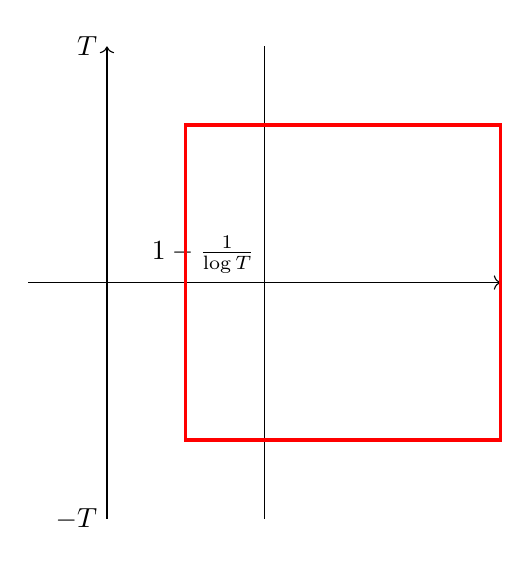
\begin{tikzpicture}
  \draw[->] (-1,0) -- (5,0);
  \draw[->] (0,-3)node[left]{$-T$} -- (0,3)node[left]{$T$};
  \draw[] (2,-3) -- (2,0)node[above left]{$1-{\frac 1 {\log T}}$} --(2,3);
  \draw[very thick, red] (1,-2) -- (1,2)
    -- (5,2) -- (5,-2) -- cycle;
\end{tikzpicture}
\end{center}
  \begin{lemma}
    $\vert\zeta(s)\vert = o(\log T), T\to \infty$. That is there are $K>0$ and $T_0$ such that for any $T\geq T_0\geq 1$, we have,
    \begin{equation*}
      \vert\zeta(s)\vert\leq K\log T.
    \end{equation*}
  \end{lemma}
  \begin{proof}
    The first statement is due to the first derivative of $\zeta$ and it is assgined as an exercise. For the second part,
    for $\Re(s),\sigma>1$, we have,
    \begin{align*}
      \zeta(s) & = \sum_{n\geq 1}{\frac 1 {n^s}},\\
      & = \sum_{n\leq T}{\frac 1 {n^s}}+\sum_{n>T}{\frac 1 {n^s}},\\
      & = \sum_{n\leq T}{\frac 1 {n^s}}-{\frac {\lfloor T\rfloor} {T^s}}+s\int_1^\infty {\frac {\lfloor t\rfloor} {t^{s+1}}}dt,\\
      & = \sum_{n\leq T}{\frac 1 {n^s}}+{\frac {T^{1-s}} {s-1}} + {\frac {\{ T\}}{T^s}}-s\int_T^\infty {\frac {\{u\}} {u^{s+1}}}du.
    \end{align*}
    Note that the right hand side is analytic where $\Re(s)>0$ and $s\not=1$. Now we will extimate the last equation above on the boundary of the red rectangle above. Let $\sigma_0 = 1-{\frac 1 {\log T}}$.
    \begin{align*}
      \left\vert\sum_{n\leq T}{\frac 1 {n^s}}\right\vert & << \int_1^T{\frac {du} {u^{\Re(s)}}},\\
      &\leq \int_1^T{\frac {du} {u^{\sigma_0}}},\\
      & = {\frac {T^{1-\sigma_0}} {1-\sigma_0}},\\
      &<<\log T.
    \end{align*}
    Observe that ,
    \begin{align*}
      1-\sigma_0 & = {\frac 1 {\log T}},\\
      T^{1-\sigma_0} & = T^{{\frac 1 {\log T}}},\\
      & = e.\\
      y & = T^{{\frac 1 {\log T}}},
      \log y &= \log T{\frac 1 {\log T}} = 1.\\
      \Rightarrow & y = e.
    \end{align*}
    We also have,
    \begin{align*}
      \left\vert{\frac {T^{1-s}} {s-1}}\right\vert & = {\frac {T^{1-\Re(s)}} {\vert s-1\vert}},\\
      & \leq {\frac {T^{1-\sigma_0}} {\vert s-1\vert}},\\
      & \leq {\frac 1 {\vert s-1\vert}},\\
      & \leq {\frac 1 {\sigma_0-1}} = \log T.
    \end{align*}
    Also consider,
    \begin{align*}
      \left\vert{\frac {\{T\}} {T}}\right\vert \leq {\frac 1 {T^{\Re(s)}}}\leq 1. 
    \end{align*}
    Finally we have,
    \begin{align*}
      & \leq \vert s\vert\int_T^\infty {\frac {du} {u^{\Re(s)+1}}},\\
      & = {\frac {\vert s\vert} {-\Re(s)u^{\Re(s)}}}\bigg{\vert}_T^\infty,\\
      & = {\frac {\vert s\vert} {\Re(s)T^{\Re(s)}}} ,\\
      & \leq {\frac {\vert s\vert} {T^{\Re(s)}}},\\
      & \leq {\frac {\sqrt{2^2+T^2}} {T^{\sigma_0}}},\\
      & << {\frac T {T^{\sigma_0}}} = T^{1-\sigma_0} = e.
    \end{align*}
    It is an exercise to check,
    \begin{align*}
      \vert \zeta'(s)\vert &\leq o((\log T)^2),\\
      \zeta'(s) & = \sum_{n\leq T}{\frac {-\log n} {n^s}}+{\frac {T^{1-s}(-\log T)} {s-1}}+T^{1-s}{\frac {-1} {(s-1)^2}} + 
    \end{align*}
    The rest is missing, check the lecture note.
  \end{proof}

  \begin{theorem}
    Let $f:n\to \C$ be an analytic, $\Lambda$ be a convex open set. Let $a,b\in\Lambda$, then ther eexists $z_1,z_2\in (a,b)$ such that 
    \begin{equation*}
      \Re(f'(z_1)) = \Re\left({\frac {f(b)-f(a)} {b-a}}\right), \Im(f'(z_2)) = \Im\left({\frac {f(b)-f(a)} {b-a}}\right).
    \end{equation*}
  \end{theorem}

  \begin{theorem}
    Ther eexists constants $c_1,c_2$ such that 
    \begin{equation*}
      1 - {\frac {c_1} {(\log T)^9}} \leq \sigma\leq 2, \vert \zeta(s)\vert >{\frac {c_2} {(\log T)^7}},
    \end{equation*}
    where $1<\vert \Im(s)\leq T$. 
  \end{theorem}

  \begin{proof}
    Recall that 
    \begin{equation*}
      \vert\zeta(\sigma)^3\zeta(\sigma+it)^4\zeta(\sigma+2it)\vert\geq 1, \sigma>1.
    \end{equation*}
    Thus we have,
    \begin{equation*}
      \vert\zeta(\sigma+it)\vert^4 \geq\vert\zeta(\sigma)\vert^3\vert\zeta(\sigma+2it)\vert^{-1},
    \end{equation*}
    $c_1$ is some (missing) constant which will be chosen later.\
    \par Fix the domain $II$ where $1+{\frac {c_1} {(\log T)^9}}\leq \sigma\leq 2$, $1\leq\vert t\vert \leq T$.
    \begin{align*}
      \zeta(s) & = {\frac s {s-1}}-s\int_1^\infty {\frac {\{u\}} {u^{s+1}}}du, \Re(s)>0, s\not =1.
      \zeta(\sigma) & = {\frac {\sigma-1+1} {\sigma-1}} - \sigma\int_1^\infty {\frac {\{u\}} {u^{t+1}}}dt.\\
      \zeta(\sigma)  & = 1+{\frac 1 {\sigma -1}}+o(1),\\
      \zeta(\sigma & << {\frac 1 {\sigma -1}}), \sigma\to 1^+,\\
      \Rightarrow & \zeta(\sigma)^{-1}>>(\sigma-1), \sigma\to 1^{+}
    \end{align*}
    We also have, 
    \begin{equation*}
      \vert\zeta(\sigma+2it)\vert  = o(\log T), 1-{\frac 1 {\log T}}
    \end{equation*}
  \end{proof}
  \begin{corollary}
    There exists some constants $C$ such that 
    \begin{equation*}
      {\frac {\zeta'(s)} {\zeta(s)}} = o((\log T)^9).
    \end{equation*}
    For $1-{\frac {c} {(\log T)^9}}\leq \Re(s)\leq 2$ and $1\leq \vert\Im(s)\vert\leq T$, we have,
    \begin{equation*}
      {\frac {\zeta'(s)} {\zeta(s)}}=\sum_{n\geq 1}{\frac {\Lambda(n)} {n^s}}.
    \end{equation*}
  \end{corollary}
  %12/4 Second part of the lecture 
  \begin{proof}
    \par Recall Cauchy's Residue theorem, suppose $f:\Omega\to\C$ is meromorphic where $\Omega$ is simply connected. 
    \begin{example}
      Halfplane $\R^n$ and $\R^n\backslash\{0\}$, for $n\geq 3$ and convex.
    \end{example}
    For $a_i,1\leq i\leq n$ poles in $U\subseteq\Omega$ simple closed curve. Then,
    \begin{equation*}
      {\frac 1 {2\pi i}}\int_U f(s)ds = \sum_{i=1}^n \Res(f,a_i)+\constant.
    \end{equation*}
    \begin{center}
  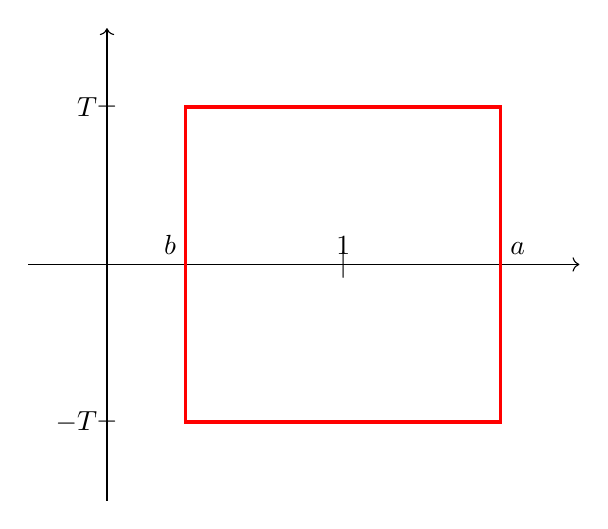
\begin{tikzpicture}
  \draw[->] (-1,0) -- (6,0);
  \draw[->] (0,-3) -- (0,3);
  \draw (0,2)node[left]{$T$};
  \draw (0,-2)node[left]{$-T$};
  \draw (0,2)node{$-$};
  \draw (0,-2)node{$-$};
  \draw[very thick, red] (1,-2) -- (1,2)
    -- (5,2) -- (5,-2) -- cycle;
  \draw (1,0)node[above left]{$b$};
  \draw (5,0)node[above right]{$a$};
\draw (3,0)node{$|$};
\draw (3,0)node[above]{$1$};
\end{tikzpicture}
\end{center}
\par where $a = {\frac 1+{\frac c {(\log(T))^9}}},b = {\frac 1-{\frac c {(\log(T))^9}}}$ $\Re(s)>0,s\not=1, \Re(s)>b$.
We claim that ${\frac {\zeta'(s)} {\zeta(s)}}$ can be analytically continued to $\Re(s)\geq b$ except simple pole at $s=i$ with residue $-1$(See lecture 5 for the justification of such poles).
\begin{align*}
  {\frac 1 {2\pi i}}\int_{R_T}{\frac {-\zeta'(s)} {\zeta(s)}}{\frac {x^s} s}ds & = \Res_{s=1}\left({\frac {-\zeta'(s)} {\zeta(s)}}\right),\\
  & = x.
\end{align*}
\par Now consider $R_T$ which is the closed path drew red in the graph.
\begin{equation*}
  \int_{R_T} = \int_{a-iT}^{a+iT}+\int_{a+iT}^{b+iT}+\int_{b+iT}^{b-iT}+\int_{b-iT}^{a-iT}.
\end{equation*}
We then have,
\begin{equation*}
  {\frac 1 {2\pi i}}\int_{a-iT}^{a+iT} {\frac {-\zeta'(s)} {\zeta(s)}}{\frac {x^s} {s}}ds = x -\int_{a+iT}^{b+iT}+\int_{b+iT}^{b-iT}+\int_{b-iT}^{a-iT}
\end{equation*}
\begin{align*}
  \left\vert{\frac 1 {2\pi i}}\int_{a+iT}^{b+iT}{\frac {-\zeta(s)}{\zeta(s)}}{\frac {x^s} {s}}ds\right\vert &= \left\vert{\frac 1 {2\pi i}}\int_a^b{\frac {-\zeta(u+iT)}{\zeta(u+iT)}}{\frac {x^{(u+iT)}} {(u+iT)}}du\right\vert,\\
  & <<\int_a^b\left\vert{\frac {-\zeta'(u+iT)} {\zeta(u+iT)}}\right\vert{\frac {x^u} {\vert u+iT\vert}}du,\\
  &\stackrel{\text{Using the previous theorem}}{<<}{\frac {\log^9T} T}x^a\int_b^a du,\\
  &<<{\frac {x^a} T}.
\end{align*}
Now we have,
\begin{align*}
  \left\vert\int_{b-iT}^{b+iT}{\frac {-\zeta'(s)} {\zeta(s)}}{\frac {x^s} {s}}ds\right\vert & = \left\vert{\frac 1 {2\pi}}\int_{-T}^T{\frac {\zeta'(b+iu)} {\zeta(b+iu)}}{\frac {x^{b+iu}} {b+iu}}du\right\vert,\\
  & << \log^9T\int_{-T}^T{\frac {x^b} {\sqrt{b^2+u^2}}}du,\\
  &<< x^b\log^9T\int_{0}^T{\frac {du} {\sqrt{b^2+u^2}}}du,\\
  & << x^b\log^9T\int_1^T{\frac {du} u},\\
  & = x^b\log^{10}T.
\end{align*}
Now back to the beginning,
\begin{equation*}
  \psi(x) = x+o({\frac {x^a} {T}}+x^b\log^{10}T)+o({\frac {x\log^2x} T}+{\frac {x^a} T}\log^9T).
\end{equation*}
Choose $T$ to be such that $2c\log x = \log^{10}T,x=e^{{\frac {\log^{10}T} x}}$.
\begin{align*}
  x^{{\frac c {\log^9T}}}=e^{{\frac {\log T} 2}} & = \sqrt{T}.\\
  x^{1-{\frac c {\log^9 T}}}\cdot\log^{10}T+{\frac {x\log^2 x} T}+{\frac {x^{1+{\frac c {\log^{9}T}}}} {T}}\log^9T&\\
  & = x\cdot T^{-{\frac 1 2}}\log^10 T+{\frac {x\log^2 x} T}+x{\frac {\sqrt{T}} T}\log^{10}T\left({\frac x {\sqrt{T}}}\right)(\log^{10}T + {\frac {\log^2x}{\sqrt{x}}}+\log^9T),\\
  &<<{\frac x {T^s}}=xe^{-c(\log x)^{{\frac 1 {10}}}}.
\end{align*}
  \end{proof}
  %12/11
\begin{definition}[Gamma function] We define the Gamma function $\Gamma:\C\to\C$ as
  \begin{equation*}
    \Gamma(s)\defeq \int_0^\infty t^{s-1}e^{-t}dt, \sigma>0.
  \end{equation*}
\end{definition}
\begin{remark}
  \begin{align*}
    \vert\Gamma(s)\vert &\leq \int_0^\infty \vert t^{s-1}\vert e^{-t}dt,\\
    & = \int_0^\infty t^{\sigma-1}e^{-t}dt,\\
    & = \left(\int_0^1+\int_1^\infty\right)t^{\sigma-1}e^{-t}dt,\\
    &\leq \int_0^1t^{\sigma-1}dt + \int_1^\infty t^{\sigma-1}e^{-t}dt, \left({\frac {t^n} {e^t}}\stackrel{t\to\infty}{\to}0\right).\\
    &<< {\frac 1 \sigma}+\int_1^\infty t^{\sigma-1}t^{-2\sigma}dt,\\
    &<< {\frac 1 \sigma}.
  \end{align*}
  \label{remark_bound_gamma}
\end{remark}

\begin{theorem}
  \begin{equation*}
    F(s) = \int f(s,t)dt.
  \end{equation*}
  $F:\Omega\to \C$ is analytic in $\Omega$ if 
  \begin{enumerate}[i).]
    \item $f(s,t)$ is continuous in $(s,t)$,
    \item $f(s,t)$ is analytic in $s$,
    \item $\int f(s,t)$ is uniformly bounded on compact subsets of $\Omega$.
  \end{enumerate}
\end{theorem}
In Remark \ref{remark_bound_gamma}, suppose $a\leq\Re(s)\leq b$ then the last two inequalities will be,
\begin{align*}
  \int_0^1t^{\sigma-1}dt + \int_1^\infty t^{\sigma-1}e^{-t}dt&\\
    &<<_b {\frac 1 \sigma}+\int_1^\infty t^{b-1}t^{-2b}dt,\\
    &<<_b {\frac 1 \sigma}+{\frac 1 b} = {\frac 1 a}+{\frac 1 b}.
\end{align*}
Thus we observe that in $\sigma>0$, using integration by parts,
\begin{align*}
  \Gamma(s+1) & = s\Gamma(s).
\end{align*}
Thus for any $n\in\N$, we have $\Gamma(n) = n!$.
We have,
\begin{equation*}
  \Gamma(s) = {\frac {\Gamma(s+1)} s},\sigma>0.
\end{equation*}
Note $\Gamma(s+1)$ is analytic if $\sigma>-1$. Thus $\Gamma(s)$ is analytic in $\sigma>-1$ except simple pole at $s=0$ with residue $1$. That is 
\begin{equation*}
  \lim_{s\to0}s\Gamma(s) = 1. 
\end{equation*}
We also have,
\begin{equation*}
  \Gamma(s) = {\frac {\Gamma(s+2)} {\Gamma(s+1)}},\sigma>0.
\end{equation*}
Note that in the numerator, we have $\sigma>-2$. $\Gamma(s)$ is analytic when $\sigma>-2$ except simple poles at $s=0,-1$ with residue 
\begin{align*}
  \lim_{s\to-1}(s+1)\Gamma(s) = {\frac {\Gamma(-1)} {-1}} = -1.
\end{align*}
Iterate the process, we have the following theorem,
\begin{theorem}
  $\Gamma(s)$ can be analytically continued to $\C$ except simple poles at $s = -k$ where $k\in\Z_{\geq 0}$ with residue ${\frac {(-1)^k} {k!}}$.
\end{theorem}
\begin{remark}
  \begin{align*}
    \Gamma(s)\Gamma(1-s) & = {\frac {\pi} {\sin\pi s}}, s\in\C.\\
    \lim_{s\to m}\Gamma(s)\Gamma(1-s)\sin\pi s = \pi s.
    \Gamma(s)\Gamma\left(s+{\frac 1 2 }\right) = \sqrt{\pi}2^{1-2s}\Gamma(2s),\forall s\in\C.
  \end{align*}
\end{remark}
\begin{exercise}
  Show 
  \begin{equation*}
    \sum_{n\in\Z}e^{-(n+\alpha){\frac \pi x}}=\sqrt{x}\sum_{n\in\Z}e^{-n^2\pi x+2\pi i n \alpha}, \forall \alpha\in i\R, x>0.
  \end{equation*}
  Note that $\sum_{n\in\Z}a_n$ is convergent if 
  \begin{equation*}
    s_N\defeq \sum_{\vert n\vert \leq N}a_n,
  \end{equation*}
  is convergent.
  \label{exercise_fourier_poisson_summation}
\end{exercise}
\begin{theorem}
  $\Gamma(s) \not=0,\forall s\in\C$.
\end{theorem}
\begin{proof}
  Note that the case when $s\in\Z$ is already shown. Thus suppose $s\not\in\Z$. If possible $\Gamma(s) = 0$. Then it will follow that $\Gamma(1-s)$ has a pole which is a contradiction.
  ${\frac 1 {\Gamma(s)}}$ has a simple zero at $s=0,-1,-2,\cdots$.\\
  \par Step 1 
  \begin{equation*}
    \Gamma\left({\frac s 2}\right) = \int_0^\infty e^{-t}s^{{\frac s 2}-1}dt, \sigma>0.
  \end{equation*}
  Replace $t=n^2\pi x,dt = n^2\pi dx$, we get,
  \begin{align*}
    \pi^{{\frac {-s} 2}}\Gamma\left({\frac s 2}\right)n^{-s} & = \int_0^\infty x^{{\frac s 2}-1}e^{-n^2\pi x}dx, \sigma>1.\\
    \pi^{{\frac {-s} 2}}\Gamma\left({\frac s 2}\right)\zeta(s) & = \sum_{n\in\N}\int_0^\infty x^{{\frac s 2}-1}e^{-n^2\pi x}dx,\\
    & = \int_0^\infty x^{{\frac s 2}-1}\left(\sum_{n\in\N}e^{-n^2\pi x}\right)dx,\\
    & = \sum_{n\in\N}\int_0^\infty\vert x^{{\frac s 2}-1}e^{-n^2\pi x}\vert dx,\\
    & = \sum_{n\in\N}\left(\int_0^\infty x^{{\frac \sigma 2}-1}e^{-n^2\pi x}dx\right),\\
    & = \sum_{n=1}^\infty \pi^{-{\frac {\sigma} 2}}\Gamma\left({\frac \sigma 2}\right)n^{-\sigma},\\
    & = \pi^{-{\frac \sigma 2}}\Gamma\left({\frac \sigma 2}\right)\zeta(s),\sigma>1,\\
    & < \infty.
    \pi^{-{\frac s 2}}\Gamma\left({\frac s 2}\right)\zeta(s) & = \int_0^\infty x^{{\frac s 2}-1}\left(\sum_{n\in\N}e^{-n^2\pi x}\right).
  \end{align*}
  \par Step 2, using Poisson summation formula and $\sigma>1$, let $F\in L^1(\R)$, ie $F:\R\to\C$ and 
  \begin{equation*}
    \int_{-\infty}^\infty \vert F(t)\vert dt<\infty.
  \end{equation*}
  We have,
  \begin{equation*}
    \sum_{n\in\Z}F(n+u)
  \end{equation*}
  is absolutely and uniformly convergent in $u$. Also we have,
  \begin{equation*}
    \sum_{n\in\Z}\vert \hat{F}(n)\vert\leq\infty,
  \end{equation*}
  then 
  \begin{equation*}
    \sum_{n\in\Z}F(n+u) = \sum_{n\in\Z}\hat{F}(n)e^{2\pi i n u}.
  \end{equation*}
  Using Exercise \ref{exercise_fourier_poisson_summation} and set $\alpha=0$, we have,
  \begin{align*}
    \sum_{n\in\Z}e^{-n^2{\frac \pi 2}} & = \sqrt{s}\sum_{n\in\Z}e^{-n^2 \pi x}.
    \sum_{n\in\Z}e^{-n^2\pi x}& << \sum_{n\in\N}e^{-n\pi x},\\
    & << \int_1^\infty e^{-\pi xt }dt,\\
    & << {\frac {e^{-\pi x}} {x}}, x>0.
  \end{align*}
  Set $\theta\defeq = \sum_{n\in\Z}e^{n^2\pi x}$ then,
  \begin{align*}
    \theta(x) &= 1+2\sum_{n\in\N}e^{-n^2\pi x}.\\
    \sum_{n\in\N}e^{-n^2\pi x}&= {\frac {\theta(x) - 1} 2}, x>0.
  \end{align*}
  Using the exercise, we have,
  \begin{equation*}
    \theta\left({\frac 1 x}\right) = \sqrt{x}\theta(x).
  \end{equation*}
  Set $w(x) \defeq {\frac {\theta(x)-1} 2}$. Thus write
  \begin{align*}
    w\left({\frac 1 x}\right) & = {\frac {\theta\left({\frac 1 x}\right)-1} 2},\\
    & = {\frac {\sqrt{x}\theta(x) - 1} 2},\\
    & = {\frac {\sqrt{x}\theta (x)-1} {2}}.\\
    w\left({\frac 1 x}\right)&= \sqrt{x}w(x)+{\frac {\sqrt{x}} 2}-{\frac 1 2}. \\
    \pi^{-{\frac 1 2}}\Gamma\left({\frac s 2}\right)\zeta(s) &= \int_0^\infty x^{{\frac s 2}-1}w(x)dx, \sigma>1.
  \end{align*}
  \par Step 3
  \begin{align*}
    \int_0^1 x^{{\frac s 2}-1}w(x)dx+\int_1^\infty x^{{\frac s 2}-1}w(x)dx.
  \end{align*}
  Taking $x = {\frac 1 y}$ and $dx = -{\frac 1 {y^2}}dy$ we have,
  \begin{align*}
    \int_1^\infty \left({\frac 1 {y^2}}\right)^{{\frac s 2}-1}w\left({\frac 1 y}\right){\frac {-1} {y^2}}dy & = \int_1^\infty y^{-{\frac s 2}}w\left({\frac 1 y}\right){\frac {dy} y},\\
    & = \int_1^\infty y^{-{\frac 1 2}}\left(\sqrt{y}w(y)+{\frac {\sqrt{y}} 2}-{\frac 1 2}\right){\frac {dy} y},\\
    & = \int_1^\infty y^{-{\frac s 2}+{\frac 1 2}}w(y){\frac {dy} y}+\int_1^\infty {\frac {y^{-{\frac s 2}+{\frac 1 2} -1 }} 2}dy - {\frac 1 2}\int_1^\infty y^{-{\frac s 2}-1}dy,\\
    & = \int_1^\infty y^{{\frac {1-s} 2}}w(y){\frac {dy} y}+{\frac 1 {s(s-1)}}+\int_1^\infty (x^{{\frac s 2}}+x^{\frac {1-s} 2})w(x){\frac {dx} x},\sigma>1.
  \end{align*}
  \par Step 4, 
  \begin{align*}
    \int_1^\infty \vert x^{{\frac s 2}}+x^{{\frac {1-s} 2}}\vert \vert w(x)\vert {\frac {dx} x} &\leq \int_1^\infty (x^{{\frac {\sigma 2}-1}}+x^{{\frac {1-\sigma} 2}-1})\vert w(x)\vert dx,\\
    &<< \int_1^\infty {\frac {(x^{{\frac \sigma 2}-1}+x^{{\frac {1-\sigma} 2}-1})} {e^{\pi x}}}dx,\sigma\in\R,\\
    &<< \int_1^\infty {\frac {e^x} {e^{\pi x}}}dx,
    & << 1.
  \end{align*}
  $\int_1^\infty \vert x^{{\frac s 2}}+x^{{\frac {1-s} 2}}\vert \vert w(x)\vert {\frac {dx} x}$ is analytic in $\C$. 
  \begin{align*}
    s(s-1)\pi^{-{\frac s 2}}\Gamma\left({\frac s 2}\right)\zeta(s) & = 1+s(s-1)\int^\infty_1(x^{{\frac s 2}} +x^{{\frac {1-s} 2}})w(x){\frac {dx} x}.
  \end{align*}
  Set $\xi(x) \defeq 1+s(s-1)\int^\infty_1(x^{{\frac s 2}} +x^{{\frac {1-s} 2}})w(x){\frac {dx} x}$, then it is entire. and for all $s$ we have,
  \begin{equation*}
    \xi(1-s)=\xi(s).
  \end{equation*}
  Thus obtain,
  \begin{equation*}
    (1-s)(1-s-1)\pi^{-{\frac {(1-s)} 2}}\Gamma\left({\frac {1-s} 2}\right) = s(s-1)\pi^{-{\frac s 2}}\Gamma\left({\frac s 2}\right)\zeta(s).
  \end{equation*}
  Using the construction of $w(s)$ we have,
  \begin{equation*}
    \vert w(x)\vert <<\vert \theta(x)\vert << {\frac {e^{-\pi x}} x},\forall x>0.
  \end{equation*}
  Also we have,
  \begin{align*}
    \zeta(1-s)&= \pi^{-s+{\frac 1 2}}{\frac {\Gamma\left({\frac s 2}\right)} {\Gamma\left({\frac {1-s} 2}\right)}}\zeta(s),\\
    \zeta(1-s) & = \pi^{-s}2^{1-s}\cos\left({\frac {\pi s} s}\right)\Gamma(s)\zeta(s).
  \end{align*}
  Note that $\zeta(s)$ has an analytic continuation to $\C$ except simple pole at $s$.
  %Missing part below
  \begin{align*}
    \lim_{s\to 1}\zeta(1-s) &= \pi^{-1}\lim_{s\to 1}{\frac {\cos{\frac {\pi s} 2} \zeta(s)(s-1)} {s-1}},\\
  \end{align*}
  \begin{align*}
    \zeta(-2n) & = 
  \end{align*}
  Recall \begin{align*}
  \zeta(s) & = \sum_{n\in\N}{\frac 1 {n^s}},\\
  & = {\frac s {s-1}}-s\int_1^\infty {\frac {\{t\}} {t^{s+1}}}dt, \sigma>0,s\not=1.
  \end{align*}
  If $s$ is real,
  \begin{align*}
  \vert \zeta(s)-{\frac s {s-1}}\vert &\leq \vert s\vert\int_1^\infty {\frac {\{t\}} {t^{\sigma+1}}}dt,
  & < {\frac {\vert s\vert }\sigma} = {\frac \sigma \sigma}=1.
  \end{align*}
  Thus we obtain,
  \begin{align*}
  -1+{\frac s {s-1}}&<\zeta(s)<1+{\frac s {s-1}}\\
    {\frac 1 {s-1}}<\zeta(s)<{\frac {2s-1} {s-1}},\\
    -1<(1-s)\zeta(s)&<1-2s<0\quad\text{ if } {\frac 1 2}<s<1\\
    \Rightarrow & \zeta(s)\not=0,\quad \text{ if } {\frac 1 2}<s<1.
  \end{align*}
\end{proof}
%1218
\begin{notation}
  Given $\chi\mod{q}$, we set,
  \begin{equation*}
    \tau(\chi) = \sum_{k=1}^q \chi(k)e^{{\frac {2\pi ik} q}}.
  \end{equation*}
\end{notation}

%Missing above,
\subsection{Primitive characters}
\begin{definition}
  A character $\chi$ is called primitive if its conductor is %missing,
\end{definition}

\begin{example}
  Take $\chi:(\Z/8\Z)^\times\to\C^times$.
\end{example}

\begin{lemma}
  Suppose $x\in\left[0,{\frac 1 2}\right]$, then 
  \begin{equation*}
    \vert\sin\pi x\vert\geq 2x.
  \end{equation*}
\end{lemma}

\begin{proof}
  Exercise.
\end{proof}

\begin{lemma}
  For $n\in \Z$, we have,
  \begin{equation*}
    \chi(n)\tau(\overline{\chi}) = \sum_{k=1}^q \overline{\chi}(k)e^{{\frac {2\pi i k} q}},
  \end{equation*}
  where $\chi$ is a primitive character modulo $q$ and $\chi\not=\chi_0$. 
\end{lemma}
\begin{proof}
  \begin{align*}
    \overline{\chi(n)}\overline{\tau(\overline{\chi})} = \sum_{l=1}^q\chi(l)e^{-{\frac {2\pi i l} q}}.
  \end{align*}
  Multiplying this equation with the one in the statement we have,
  \begin{equation*}
    \vert \chi(n)\vert^2\vert \tau(\overline{\chi})\vert^2 = \sum_{k,l=1}^q \overline{\chi(k)}\chi(l)e^{{\frac {2\pi i (k-l)} q}}.
  \end{equation*}
  Applying $\sum_{n\leq x}$ to the both sides of the above equation, we have,
  \begin{align*}
    \vert\tau(\overline{\chi})\vert^2\sum_{n\leq x}\vert\chi(n)\vert^2 = \sum_{k,l=1}^q\overline{\chi(k)}\chi(l)\left(\sum_{n\leq x}\left(e^{{\frac {2\pi i(k-l)} q}}\right)^n\right).
  \end{align*}
  Note that 
  \begin{align*}
    x+x^2+\cdots+x^q = \begin{cases}
      {\frac {x(x^q-1)} {x-1}}, (x\not =1),\\
      q, (x=1),
    \end{cases}\\
    & = \begin{cases}
      0, (x\not =1, x^q = 1),\\
      q, (x=1),
    \end{cases}\\
  \end{align*}
  Take $x = e^{{\frac {2\pi i (k-l)} q}} = \cos{\frac {2\pi} q}(k-l)+i\sin{\frac {2\pi} q}(k-l)=1$. $x=1$ if and only if $q|k-l$ thus 
  \begin{equation*}
    \sum_{n\leq x}\left(e^{{\frac {2\pi i(k-l)} q}}\right)^n = \begin{cases}
      0,(q\not|k-l),\\
      q,(\text{otherwise}).
    \end{cases}
  \end{equation*}
  Therefore, we get,
  \begin{align*}
    \vert\tau (\overline{\chi})\vert^@\sum_{n\leq x}\vert\chi(n)\vert^2 & = q\sum_{\substack{k,l=1\\ q|k-l}}^q \overline{\chi}(k)\chi(l),\\
    & = q\sum_{k=1}^q\overline{\chi}(k)\chi(k),\\
    & = q\sum_{k=1}^q \vert \chi(k)\vert^2.
  \end{align*} 
  Therefore $\vert\tau(\overline{\chi})\vert^2 = q,\vert\tau\vert = \sqrt{q}$.
  \par Consider $(n,q)=1$, then 
  \begin{align*}
    \chi(n)\tau(\overline{\chi}) & = \chi(n)\sum_{k=1}^q\overline{\chi}(k)e^{{\frac {2\pi i k} q}},\\
    & = \chi(n)\sum_{\substack{k=1\\(k,q)=1}}^q\overline{\chi}(k)\chi(k)e^{{\frac {2\pi i k} q}},\\
  \end{align*}
  Set $k = nt$, we get,
  \begin{align*}
    \chi(n)\tau(\overline{\chi}) & = \sum_{\substack{t=1\\ (t,q)=1}}^q\overline{\chi}(nt)\chi(n)e^{{\frac {2\pi i nt} q}}.\\
    \overline{\chi}(nt) & = \overline{\chi}(n)\overline{\chi}(t).\\
    \chi(n)\tau(\overline{\chi}) & = \sum_{\substack{t=1\\ (t,q)=1}}^q\overline{\chi}(t)e^{{\frac {2\pi i nt} q}}.
  \end{align*}
  Observe that 
  \begin{align*}
    \tau(\overline{\chi})\left(\sum_{n\leq x}\chi(n)\right) & = \sum_{k=1}^{q-1}\overline{\chi}(k)\left(\sum_{n\leq x}e^{{\frac {2\pi i kn} q}}\right),\\
    \vert\tau(\overline{\chi})\vert\cdot\vert\sum_{n\leq x}\chi(n)\vert & \leq \sum_{k=1}^{q-1}\left\vert\sum_{n\leq x}e^{{\frac 2\pi i kn} q}\right\vert,\\
    & = \sum_{k=1}^{q-1}\left\vert{\frac {e^{{\frac {2\pi i k} q}}\left(e^{{\frac {2\pi in[x]} q}}-1\right)} {e^{{\frac 2\pi i k} q} - 1}}\right\vert,\\
    &\leq \sum_{k=1}^{q-1}{\frac 2 {\vert e^{{\frac {2\pi k} q}}-1\vert}},\\
  \end{align*}
  Note that for all $y\in i\R$,
  \begin{align*}
    2 i\sin y &= e^{-iy}(e^{2iy}-1),\\
    \vert 2\sin y\vert & = \vert e^{2iy}-1\vert.
  \end{align*}
  Apply this to the equation above we have,
  \begin{equation*}
    \sum_{k=1}^{q-1}{\frac 2 {\vert e^{{\frac {2\pi k} q}}-1\vert}} = \sum_{k=1}^{q-1}{\frac 1 {\vert\sin{\frac {\pi k} q}\vert}}.
  \end{equation*}
  Using the lemma, we get,
  \begin{align*}
    \sum_{k=1}^{q-1}{\frac 1 {\vert\sin{\frac {\pi k} q}\vert}} & = \sum_{1\leq k\leq{\frac q 2}}{\frac 1 {\vert\sin{\frac {\pi k} q}\vert}}+\sum_{{\frac q 2}<k}^{q-1}{\frac 1 {\vert\sin{\frac {\pi k} q}\vert}}.
    & = 2\sum_{1\leq k\leq{\frac q 2}}{\frac 1 {\vert\sin{\frac {\pi k} q}\vert}},\\
    &\leq \sum_{1\leq k\leq{\frac q 2}}{\frac k q} << q\log{\frac q 2}<<q\log q.
  \end{align*}
  Thus we conclude $\vert(\overline{\chi})<<\sqrt{q}$ if $\chi$ is primitive and $q>1$, we have,
  \begin{equation*}
    \left\vert\sum_{n\leq x}\chi(n)\right\vert<<\sqrt{q}\log q,
  \end{equation*}
  uniformly in $q$ as $x\to\infty$.
\end{proof}
$L(q,\chi)$ functional equation, where $\chi\not=\chi_0$ and $\chi$ is primitive. Suppose $\chi(-1)=1$ that is it is an even character.
From previous discussion, we have,
\begin{equation*}
  \pi^{-{\frac s 2}}\Gamma\left({\frac s 2}\right)n^{-s} = \int_0^\infty x^{{\frac s 2}}e^{-n^2\pi x}{\frac {dx} x}.
\end{equation*}
Replace $x$ with ${\frac x q}$ and $\sigma>0$, we habe,
\begin{equation*}
  \pi^{-{\frac s 2}}q^{{\frac s 2}}\Gamma\left({\frac s 1}\right)n^{-s} = \int_0^\infty x^{{\frac s 2}}e{-n^2\pi x}{\frac {dx} x},\sigma>0.
\end{equation*}
For $\sigma>1$, we have,
\begin{align*}
  \pi^{-{\frac s 2}}q^{{\frac s 2}}\Gamma\left({\frac s 2}\right)L(s,\chi)& = \sum_{n=1}^\infty\int_0^\infty \chi(n)x^{{\frac s 2}}e^{-n^2{\frac {\pi x} q}}{\frac {dx} x},\\
  & = \int_0^\infty x^{{\frac s 2}}\left(\sum_{n=1}^\infty \chi(n)e^{-n^2{\frac {\pi x} q}}\right){\frac {dx} x}, \sigma>1.
\end{align*}
Let 
\begin{equation*}
  \theta(x,\chi)  = \sum_{n\in\Z}\chi(n)e^{-{\frac {n^2\pi x} q}} = 2\sum_{n=1}^\infty\chi(n)e^{-{\frac {n^2\pi x} q}},(x>0).
\end{equation*}
Using this, we get,
\begin{align*}
  \int_0^\infty x^{{\frac s 2}}e{-n^2\pi x}{\frac {dx} x} & = {\frac 1 2}\int_0^\infty x^{{\frac s 2}}\theta(x,\chi){\frac {dx} x}, (\sigma>1).
\end{align*}
Split the integral into $\int_0^1,\int_1^\infty$.
\begin{align*}
  \tau(\overline{\chi})\theta(x,\chi) &= \left({\frac q x}\right)^{{\frac 1 2}}\theta(x^{-1},\overline{\chi}),\\
  & = \sum_{n\in\Z}(\tau(\overline{\chi})\chi(n))e^{{\frac {-n^2\pi x} q}},\\
  & = \sum_{n\in\Z}\sum_{k=1}^q\overline{\chi}(k)e^{{\frac {2\pi i nk} q}}e^{-{\frac {n^2\pi x} q}},\\
  & = \sum_{k=1}^q\overline{\chi(k)}\sum_{n\in\Z}e^{{\frac {2\pi kn} q} - n^2{\frac {\pi x} q}},\\
  &\stackrel{\text{From Lecture 7 page 6}}{=}\sum_{k=1}^q\overline{\chi}(k)\left({\frac x q}\right)^{-{\frac 1 2}}\sum_{n\in\Z}e^{-\left(m+{\frac m q}\right){\frac {\pi q} x}},\\
  & = \left({\frac q x}\right)^{{\frac 1 2}}\sum_{k=1}^q\overline{\chi}(k)\sum_{n\in\Z}e^{-\left(m+{\frac m q}\right){\frac {\pi q} x}}.
\end{align*}
Put $qn+m = t$, then 
\begin{equation*}
  \overline{\chi}(qn+m) = \overline{\chi}(m) = \overline{\chi}(t).
\end{equation*}
Thus,
\begin{align*}
  \left({\frac q x}\right)^{{\frac 1 2}}\sum_{k=1}^q\overline{\chi}(k)\sum_{n\in\Z}e^{-\left(m+{\frac m q}\right){\frac {\pi q} x}} & = \left({\frac q x}\right)^{\frac 1 2}\sum_{t\in\Z}\overline{\chi}(t)e^{-{\frac {t^2\pi} {qx}}}= \left({\frac q x}\right)^{{\frac 1 2}}\theta(x^{-1},\overline{\chi}).
\end{align*}
Now for the splitted integral, we have,
\begin{align*}
  {\frac 1 2}\int_0^1x^{{\frac s 2}}\theta(x,\chi){\frac {dx} x}+{\frac 1 2}\int_1^\infty \int_0^1x^{{\frac s 2}}\theta(x,\chi){\frac {dx} x}{\frac {dx} x}.
\end{align*}
Replacing $x$ with ${\frac 1 x}$, we get, 
\begin{align*}
  & = {\frac {\tau(\chi)} {2\sqrt{q}}}\int_1^\infty x^{{\frac {1-s} 2}}\theta(x,\overline{\chi}){\frac {dx} x}+{\frac 1 2}\int_1^\infty \int_0^1x^{{\frac s 2}}\theta(x,\chi){\frac {dx} x}.
\end{align*}
Set 
\begin{equation*}
  \xi(s,\chi) \defeq {\frac {\tau(\chi)} {2\sqrt{q}}}\int_1^\infty x^{{\frac {1-s} 2}}\theta(x,\overline{\chi}){\frac {dx} x}+{\frac 1 2}\int_1^\infty \int_0^1x^{{\frac s 2}}\theta(x,\chi){\frac {dx} x}.
\end{equation*}
Use that $\theta(x,\overline{\chi})<<e^{-{\frac {\pi x} q}}$ and $\vert\tau(\chi)\vert=\sqrt{q}$. It turns out that $\xi$ is uniformly bounded on compact subsets of $\C$ and in particular, this is entire.
\begin{lemma}
  \begin{equation*}
    \xi(1-s,\chi) = {\frac {\tau(\chi)} {\sqrt{q}}}\xi(s,\overline{\chi}).
  \end{equation*}
\end{lemma} 
\begin{proof}
  Recall,
  \begin{equation*}
    \tau(\overline{\chi})\theta(x,\chi) =\left({\frac q x}\right)^{{\frac 1 2}}\theta(x^{-1},\overline{\chi}),
  \end{equation*}
  and 
  \begin{equation*}
    \vert\tau(\chi)\vert^2 = q.
  \end{equation*}
  We get,
  \begin{equation*}
    {\frac {\tau(\chi)} {\sqrt{q}}} = {\frac {\sqrt{q}} {\overline{\tau(\chi)}}}={\frac {\sqrt{q}} {\tau(\overline{\chi})}}.
  \end{equation*}
  Then,
  \begin{equation*}
    L(1-s,\chi) = {\frac {\tau(\chi)} {q^{1-s}}}\pi^{-s}2^{1-s}\cos{\frac {\pi s} 2}(\Gamma(s))L(s,\overline{\chi}).
  \end{equation*}
  Note that $\chi(-1) = 1$ and is primitive (in the case of odd integer replace $\cos$ with $\sin$).
  Note also that 
  \begin{enumerate}[i).]
    \item $L(s,\chi) = 0,s=0,-2,-4,\cdots$ when $\chi$ is even,
    \item $L(s,\chi) = -1,-3,-5,\cdots$ when $\chi$ is odd.
  \end{enumerate}
  When $0<\sigma<1$, 
\end{proof}
\end{document}